\documentclass{article}

\usepackage[a4paper]{geometry}
\usepackage[ngerman]{babel}
\usepackage[utf8]{inputenc}
\usepackage[T1]{fontenc}
\usepackage{graphicx}
\usepackage{fancyhdr}
\usepackage{xcolor}
\usepackage{float}
\usepackage{hyperref}

\graphicspath{{./images/}}

\pagestyle{fancyplain}
\fancyhf{}
\lhead{\fancyplain{}{Gruppe 11 – Mathias Baumbach \& Mara Schulke} }
\rhead{\fancyplain{}{\today}}
\cfoot{\fancyplain{}{\thepage}}

\begin{document}

\begin{titlepage}
	\begin{flushleft}
		TH Brandenburg \\
		Online Studiengang IT Sicherheit \\
		Fachbereich Informatik und Medien \\
		Netzwerksicherheit \\
		Prof.\ Dr.\ Michael Pilgermann
	\end{flushleft}

	\vfill

	\begin{center}
		\Large{Einsendeaufgabe 1}\\[0.5em]
		\large{Wintersemester 2023}\\[0.25em]
		\large{Abgabetermin \today}
	\end{center}

	\vfill

	\begin{flushright}
		Gruppe 11 \\
		Mathias Baumbach (Matr-Nr. 20213703) \\
		Mara Schulke (Matr-Nr. 20215853)
	\end{flushright}
\end{titlepage}

\begin{abstract}
	Innerhalb dieser Einsendeaufgabe werden verschiedene Aspekte der Netzwerksicherheit – vor 
	allem aus der Angreiferperspektive – betrachtet. Im Rahmen der Bearbeitung konnten wir 
	wertvolle Erfahrungen sammeln – gerade die Aufgabe 2.5 (Google-Hacking) hat uns erneut vor 
	Augen geführt wie wichtig eine entsprechende Absicherung von IT-Systemen ist, da wir 
	innerhalb von wenigen Minuten vollen Zugriff auf die Datenbank eines PHP Web-Servers 
	erlangen konnten. Wir haben den Betreiber informiert und anonymisiert. So, dass diese 
	Dokumentation nicht zu einer weiteren Ausnutzung verwendet werden kann.
\end{abstract}

\tableofcontents

\listoffigures

\newpage

\section{Vorbereitungen}

Die bevorzugte Methode zur Beantwortung der Einsendeaufgabe besteht darin, dass Sie 
entweder ParrotOS oder Kali Linux als virtuelle Maschine auf Ihrem Rechner installieren. 
Diese beiden Linux-Distributionen sind speziell auf die IT-Sicherheit ausgelegt und haben 
daher viele interessante Tools schon vorinstalliert. 
Tipp zur Durchführung: Laden Sie von ParrotOS  eine .ova für virtuelle Maschinen herunter 
(genauer die .ova der Security Edition; Tipp: das Superuser-Password lautet dann "parrot" 
und nicht "toor" wie bei anderen Versionen). Falls noch nicht vorhanden, installieren Sie 
Virtualbox  und führen die virtuelle Maschine darin aus.
Leider gibt es in der letzten Zeit zunehmend Prozessorarchitekturen (gerade für Mac), bei 
denen keine Möglichkeit zum Betrieb von virtuellen Maschinen besteht. Sollte das der Fall 
sein, dann bearbeiten Sie die Aufgaben auf Ihrem eigenen Betriebssystem. Sie müssen dafür 
die Tools einzeln herunterladen.

\newpage

\section{Durchführung}

\subsection{Telnet und Wireshark}

\subsubsection*{Aufgabenstellung}

Wireshark ist bei ParrotOS und Kali Linux vorinstalliert. Es kann ansonsten von der 
Wireshark-Seite heruntergeladen werden. In der Wireshark-Datei im Kurs (telnet.pcapng) ist 
eine Aufzeichnung eines Einlog-Vorgangs mit Telnet zu finden. Suchen Sie darin das 
Passwort.

\subsubsection*{Antwort}

Nach dem wir die Datei analysiert und den Telnet-Login-Vorgang bei dem Paket 
22 lokalisiert haben, konnten wir den Start des Passwords in Text-Form 
bei dem Paket 23 entdeckend. (Siehe Abb. 1).

\begin{figure}[H]
	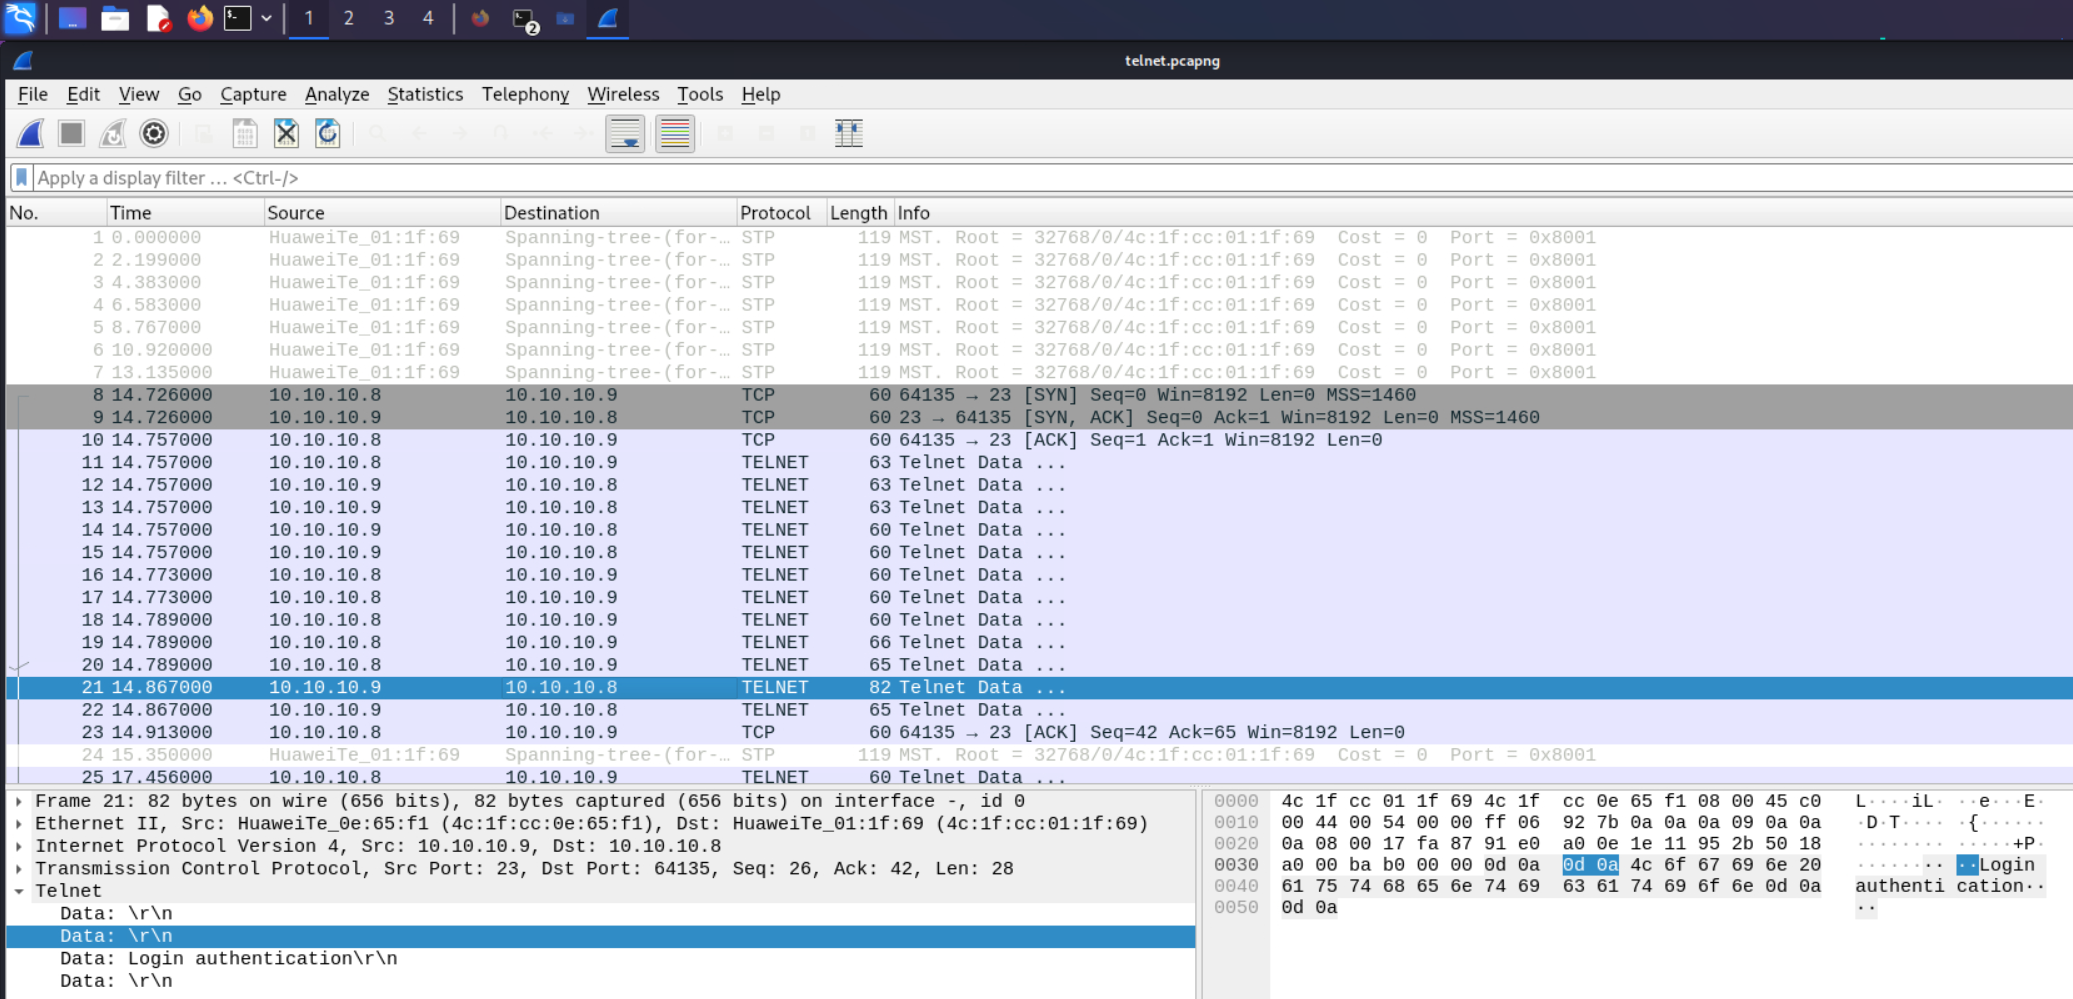
\includegraphics[width=0.75\textwidth]{images/01}
	\centering
	\caption{Telnet Datei: Start des Logins}
\end{figure}

Nun enthielt jedes weitere Paket ein Zeichen des Passworts, bis die End-Sequenz
in dem Paket 46 gesendet wurde. Zusammengesetzt ergibt dies das 
Passwort \texttt{sshnutzen}. (Siehe Abb. 2).

\begin{figure}[H]
	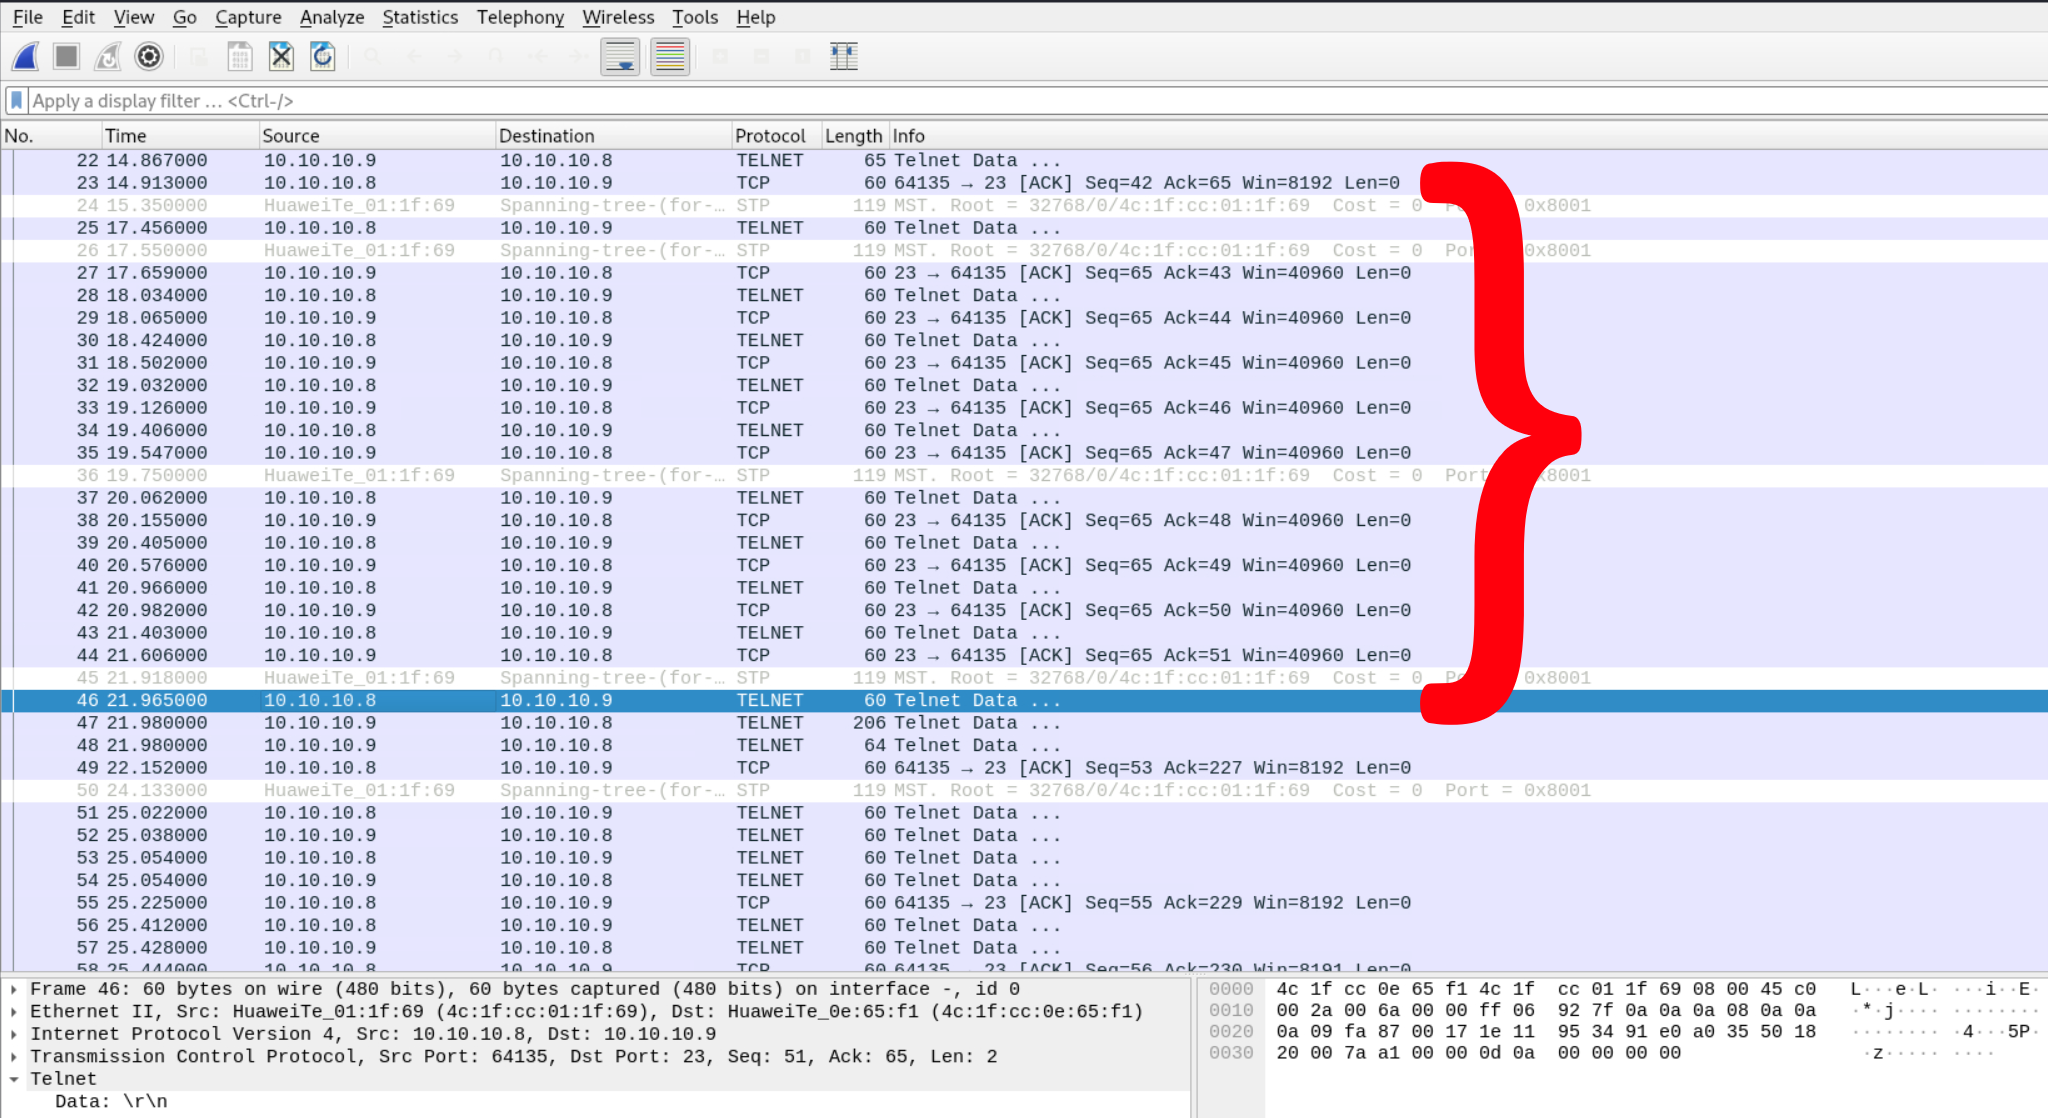
\includegraphics[width=0.75\textwidth]{images/02}
	\centering
	\caption{Telnet Datei: Login Sequenz Dauer}
\end{figure}

\newpage

\subsection{Schwachstellenscan I}

\subsubsection*{Aufgabenstellung}

Verwenden Sie \texttt{nmap} (bei ParrotOS und Kali Linux vorinstalliert), um verschiedene 
Scans des Testservers nwsmooc.mooin.org durchzuführen. Erklären Sie die Ergebnisse, wobei 
mindestens drei Tests mit jeweils unterschiedlichen Parametern durchgeführt werden müssen. 
Versuchen Sie dabei u.a. herauszufinden, welche Dienste auf dem Zielserver installiert
sind und welches Betriebssystem verwendet wird.

\subsubsection*{Antwort}

Der Aufgabe entsprechend haben wir drei sinnvolle \texttt{nmap} scans durchgeführt.
Auf den im Internet verfügbaren ubuntu manpage Seiten sind verschiedene Scan-Techniken mit
\texttt{nmap} aufgelistet. (Siehe Abb. 3).

\begin{figure}[H]
	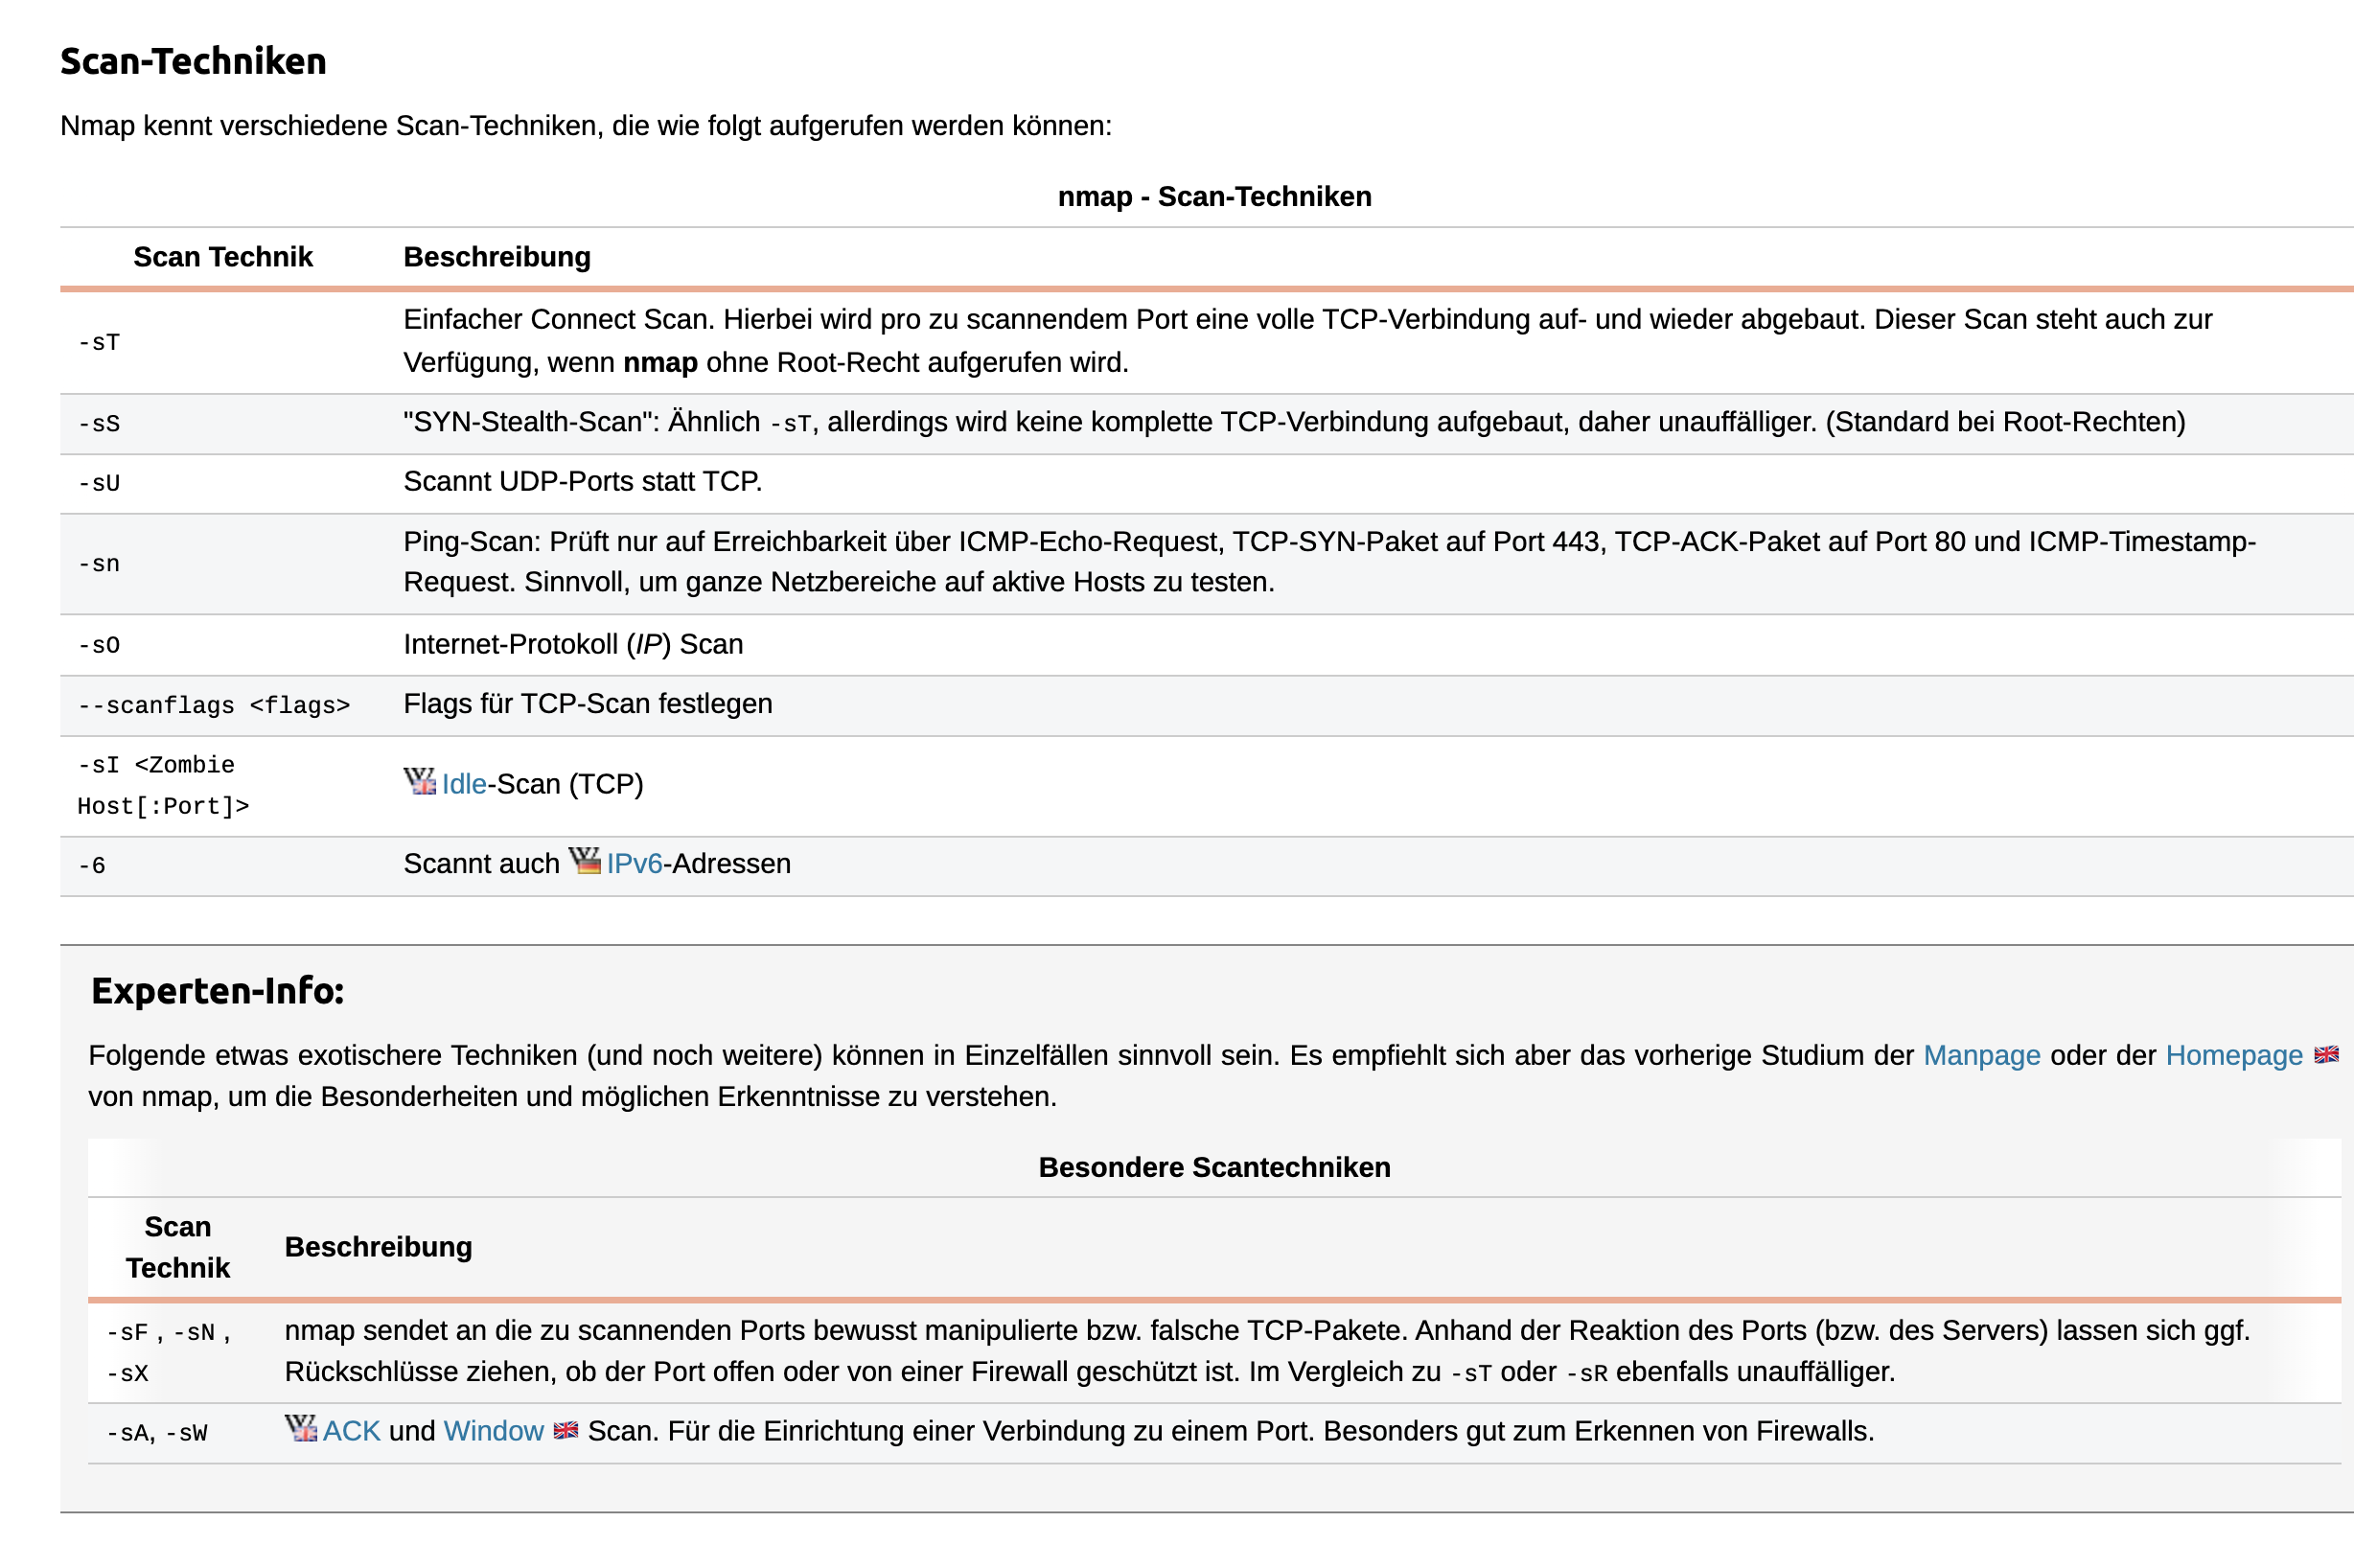
\includegraphics[width=0.75\textwidth]{images/03}
	\centering
	\caption{nmap: Scan-Techniken}
\end{figure}

Nach kurzer Recherche haben wir uns für die folgenden vier Scan-Techniken entschieden, da sie in 
Kombinationen eine gute Aussage-Stärke über das Host-System des Servers und die darauf ausgeführten
Programme treffen.

\subsubsection*{Port Scan}

Eine der bekanntesten Techniken mit \texttt{nmap} ist der Port-Scan – dieser kann entweder auf die
``well-known'' Ports beschränkt werden, oder über alle ports von 0-65536 ausgeführt werden. Da wir 
im Rahmen dieser Aufgabe eine Aussage über die Dienste des Servers treffen sollen, haben wir uns dafür
entschieden einen kompletten Port-Scan auszuführen. (Siehe Abb. 4)

\begin{figure}[H]
	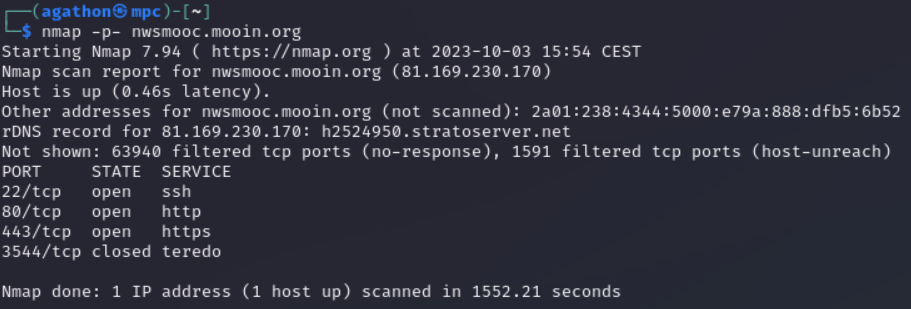
\includegraphics[width=0.75\textwidth]{images/04}
	\centering
	\caption{nmap: Port Scan}
\end{figure}

Hier lässt sich erkennen, dass der Server einen SSH-Server, einen HTTP- bzw. HTTPS-Server betreibt.
Diese Server sind öffentlich und für das Internet zugänglich. Auf dem Port 3544 wird vermutlich eine
Torredo-Instanz ausgeführt, \texttt{nmap} kann aber keine genaue Aussage darüber treffen, ob dieser
Dienst wirklich aktiv ist (daher wurde dieser Port als \texttt{CLOSED} markiert).

\subsubsection*{TCP Scan}

Als nächstes haben wir einen tiefgreifenden TCP-Scan ausgeführt, um detailiertere Informationen über
die drei (im vorherigen Schritt entdeckte) Dienste herauszufinden. (Siehe Abb. 5)

\begin{figure}[H]
	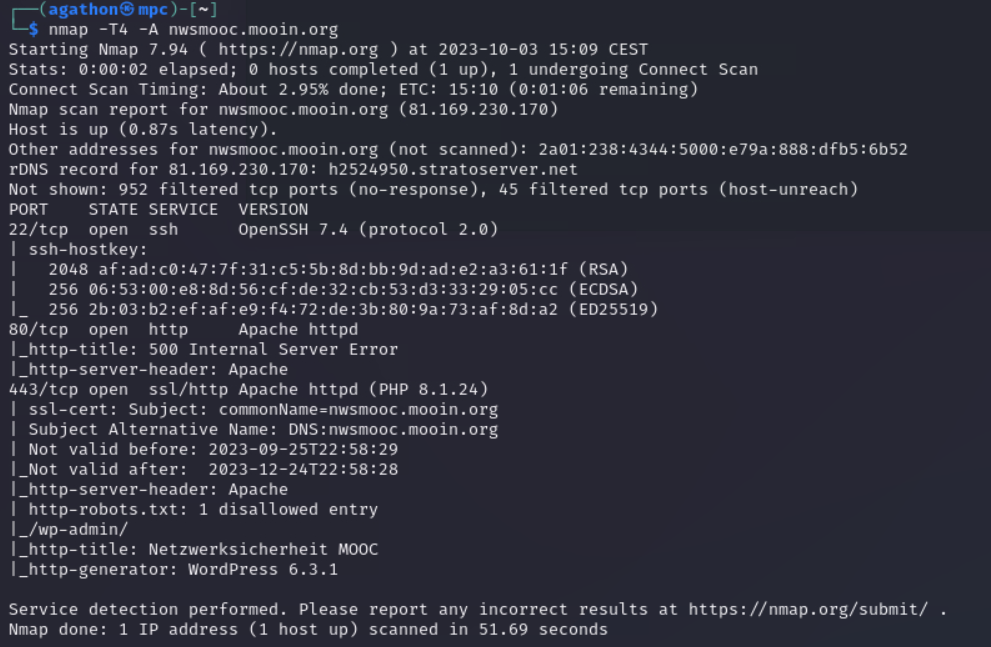
\includegraphics[width=0.75\textwidth]{images/05}
	\centering
	\caption{nmap: TCP Scan}
\end{figure}

In diesem Scan konnten wir weitere Informationen herausfinden, wie z.B. die Versionen / Distributionen
des SSH- und HTTP-Servers, die öffentlichen SSH-Schlüssel des Servers und die Konfiguration des Apache-
Servers.

\subsubsection*{Betriebsystem Scan}

Um eine Aussage über das ausgeführte Betriebssystem treffen zu können, bietet \texttt{nmap} einen 
dedizierten Betriebssystem-Scan an – dieser kann durch \texttt{-O} gestartet werden. (Siehe Abb. 6)

\begin{figure}[H]
	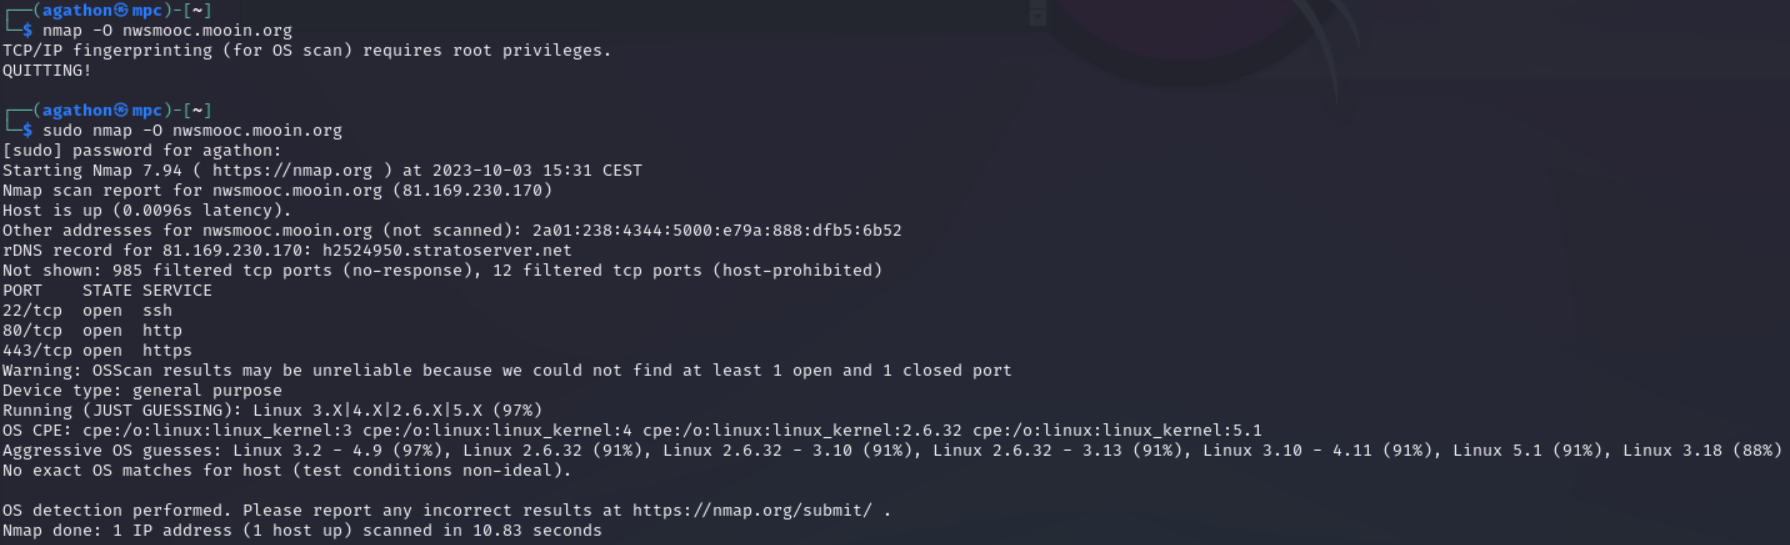
\includegraphics[width=0.75\textwidth]{images/06}
	\centering
	\caption{nmap: OS Scan}
\end{figure}

Das Ergebnis dieses Scans ist zwar nicht eindeutig, lässt aber darauf deuten, dass der Server eine Linux-
Distribution ausführt.

\subsubsection*{UDP Scan}

Zuletzt haben wir noch die bisher wenig betrachteten UDP-Dienste des Servers gescannt. (Siehe Abb. 7)

\begin{figure}[H]
	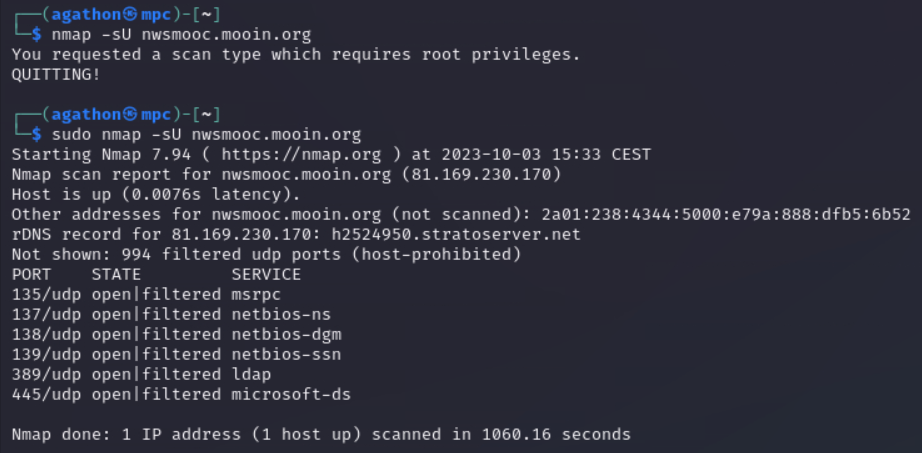
\includegraphics[width=0.75\textwidth]{images/07}
	\centering
	\caption{nmap: UDP Scan}
\end{figure}

Hierbei wurden mehrere Dienste gefunden. Zwei der 4 UDP-Dienste stehen in Verbindung mit Microsoft,
was entweder auf eine Windows-basierte Firewall oder einen Irrtum bei dem Betriebsystems-Scan hindeutet.

Jeder Dienst hat den Status \texttt{open|filtered}, was auf eine aktive Firewall-Konfiguration hindeutet.

\newpage

\subsection{MAC Spoofing}

\subsubsection*{Aufgabenstellung}

Ebenfalls bereits bei ParrotOS und Kali schon vorinstalliert ist das Tool 
\texttt{macchanger}. Machen Sie sich mit dessen Möglichkeiten vertraut, wobei z.B. ein 
Video von HackerSploit nützlich sein kann: \url{https://www.youtube.com/watch?v=bshXz5r-CQA.}
Senden Sie anschließend Datenverkehr mit gefälschter MAC-Adresse und zeichnen diesen mit 
Wireshark auf. Fertigen Sie geeignete Screenshots mit Erklärungen (wie müsste es richtig 
sein? wo ist die gefälschte MAC-Adresse in Wireshark zu sehen?) dazu an.
Mac- und Linux-Nutzer verwenden für die Aufgabe ebenfalls \texttt{macchanger} oder 
\texttt{ifconfig}. Windows-Nutzer schauen sich bitte das Youtube-Tutorial an:
\url{https://www.youtube.com/watch?v=V3Pcc8b_m0U.}
Hinweis: Bei der ersten Methode heißt der Eintrag in den erweiterten Einstellungen nicht
"Network Address", sondern "Locally Administered Address".

\subsubsection*{Antwort}

Um die MAC-Adresse unter Kali-Linux zu ändern genügte eine einfache Kombination aus dem 
Programm \texttt{macchanger} und \texttt{ifconfig}. Zu erst, um eine erfolgreiche Änderung 
bzw. ein erfolgreiches Spoofing feststellen zu können, haben wir den Netzwerk-Verkehr zum 
Web-Server der vorherigen Aufgaben aufgezeichnet. (Siehe Abb. 8)

\begin{figure}[H]
	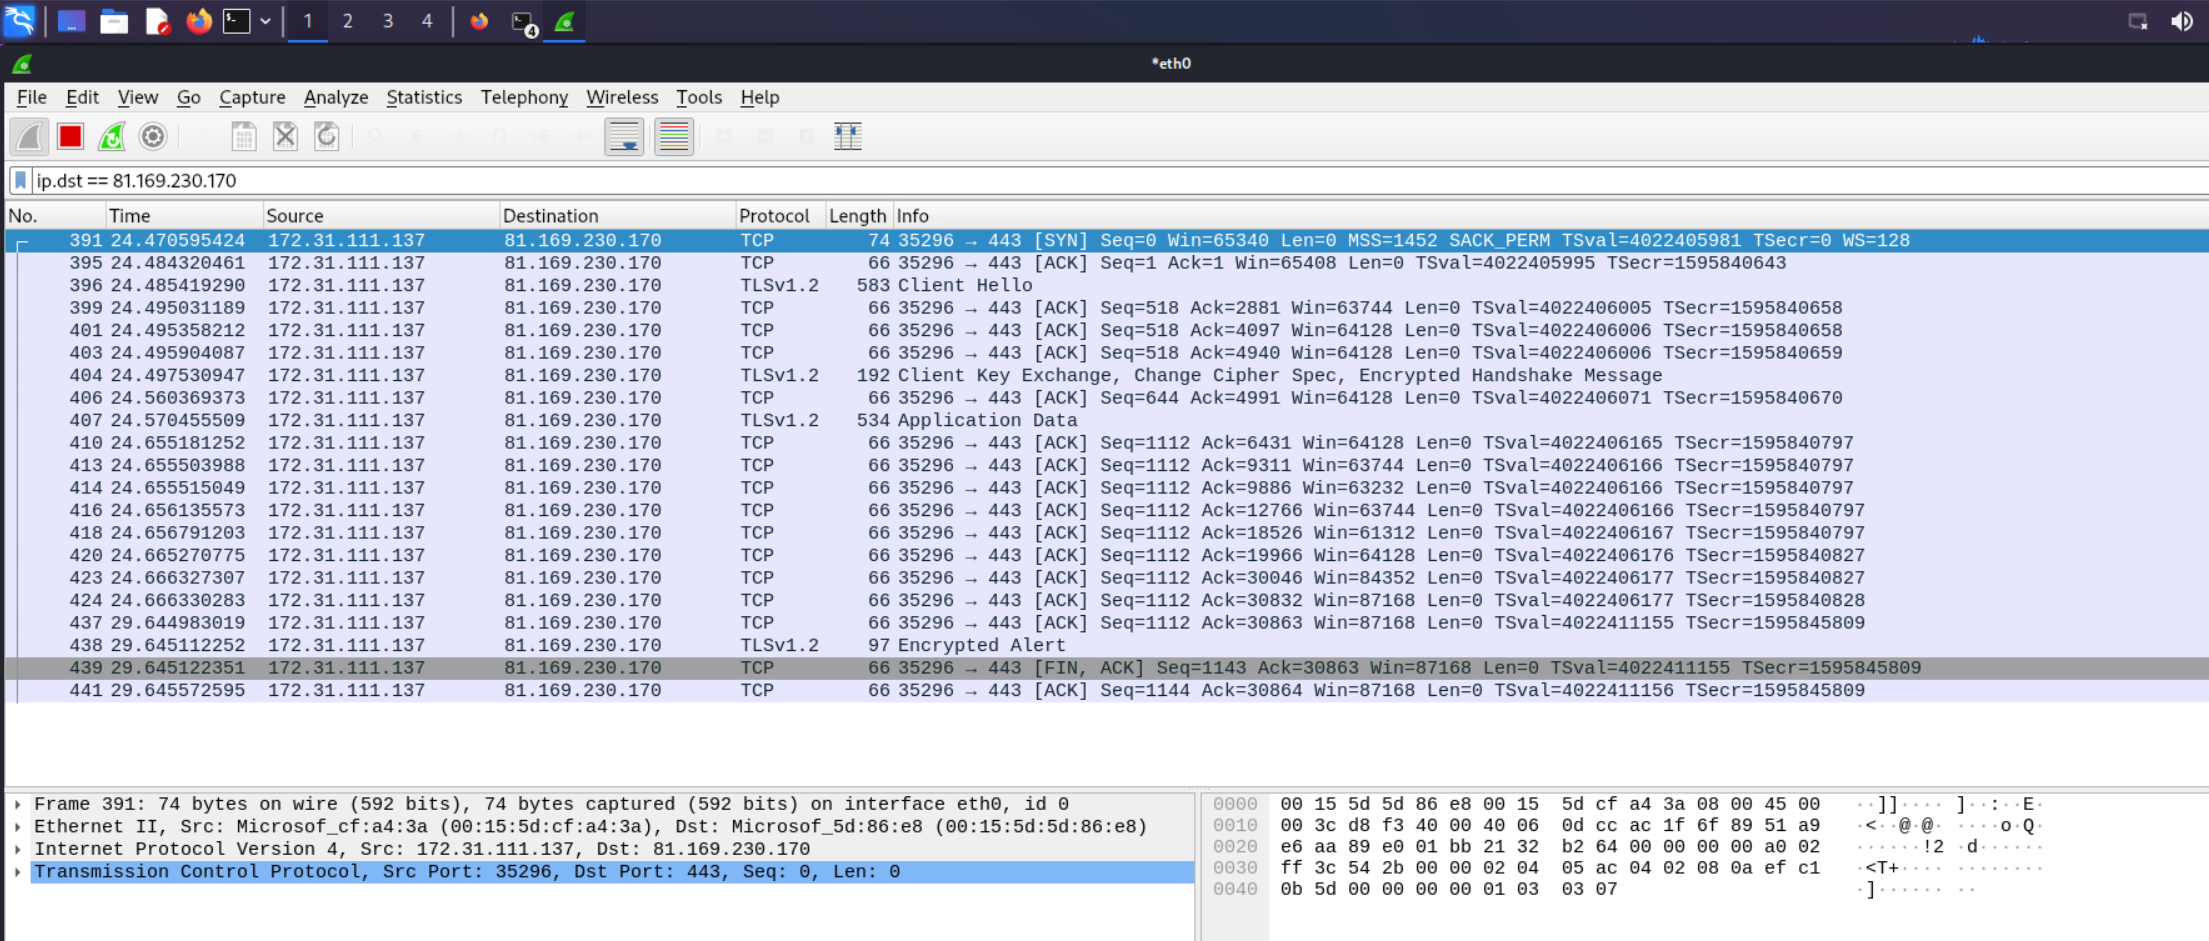
\includegraphics[width=0.75\textwidth]{images/08}
	\centering
	\caption{macspoofing: Ursprünglicher Netzwerk-Verkehr}
\end{figure}

Anschließend haben wir mittels \texttt{ifconfig} auf dem Host und in der virtuellen Maschine
die MAC-Adressen ausgelesen und mit dem Ethernet-Adressen aus dem aufgezeichneten Netzwerk-Verkehr
in Verbindung gebracht. (Siehe Abb. 9)

Die Source-Adresse (\texttt{eth0} in der VM) lautet: \texttt{00:15:5d:cf:a4:3a}

Die Source-Adresse (\texttt{WSL} auf dem Host) lautet: \texttt{00:15:5d:5d:86:e8}

\begin{figure}[H]
	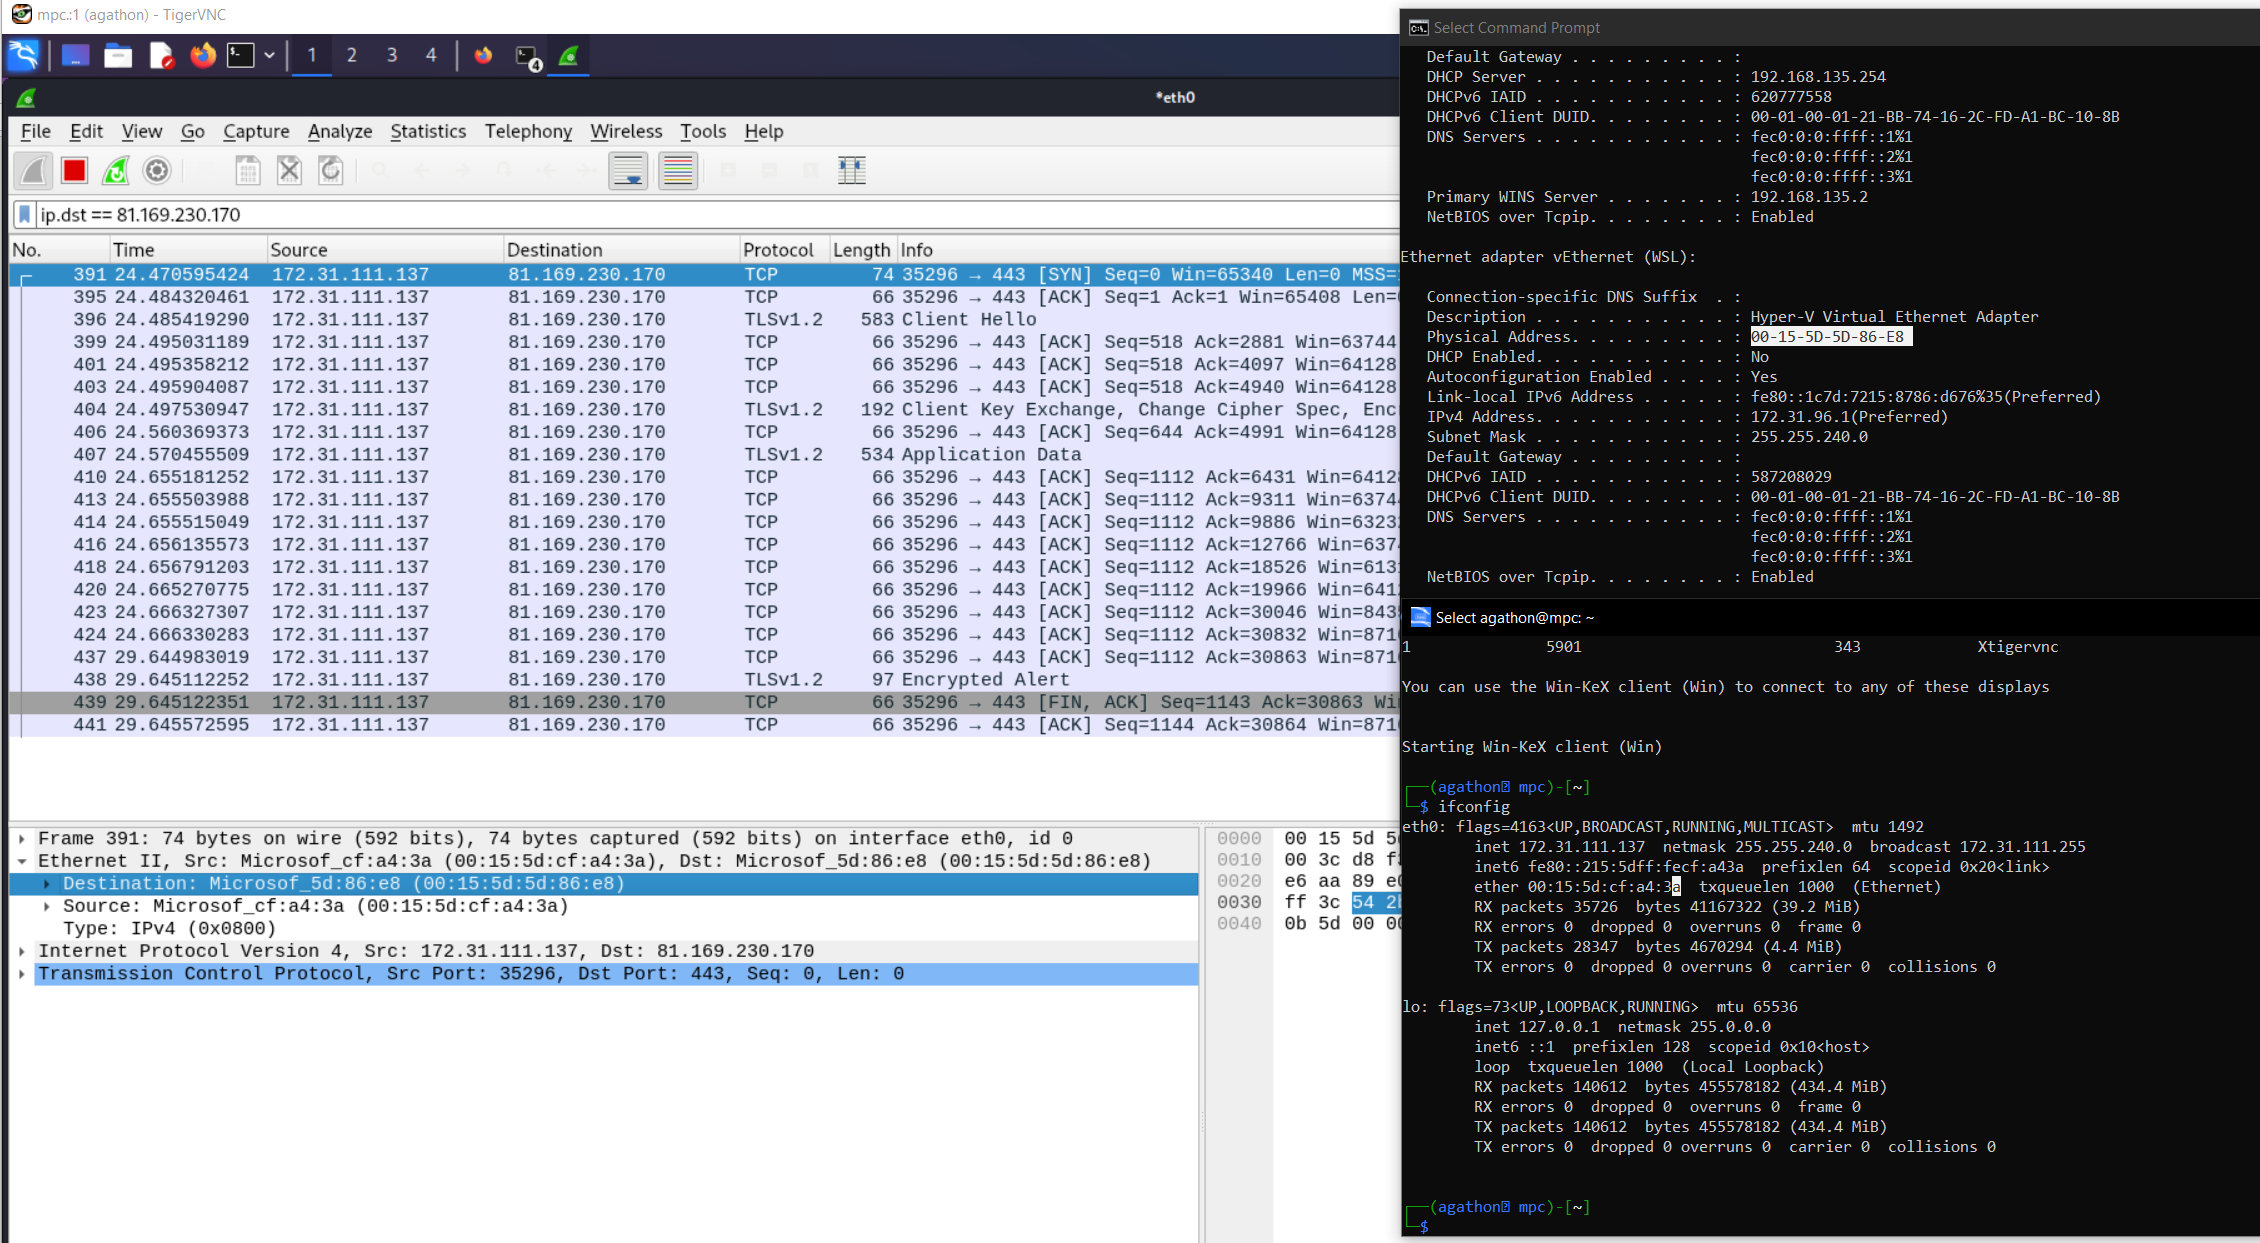
\includegraphics[width=0.75\textwidth]{images/09}
	\centering
	\caption{macspoofing: Ursprüngliche Source und Destination}
\end{figure}

In den beiden Screenshots ist zu erkennen, dass die momentane MAC-Adresse der virtuellen
Maschine \texttt{00:15:5d:cf:a4:3a} entspricht.

Nun muss zu erst das \texttt{eth0} Interface mittels \texttt{ifconfig} deaktiviert werden. 
Anschließend kann die MAC-Adresse mittels \texttt{macchanger} geändert werden. In diesem 
Beispiel haben wir lediglich die Hersteller-Nummer von \texttt{cf:a4:3a} zu \texttt{cf:a4:01}
geändert und die Vendor-ID belassen, da eine Änderung dieser zu Problemen mit den Treibern
führen kann. Anschließend muss das Netzwerk-Interface erneut durch \texttt{ifconfig} gestartet werden.
(Siehe Abb. 10)

\begin{figure}[H]
	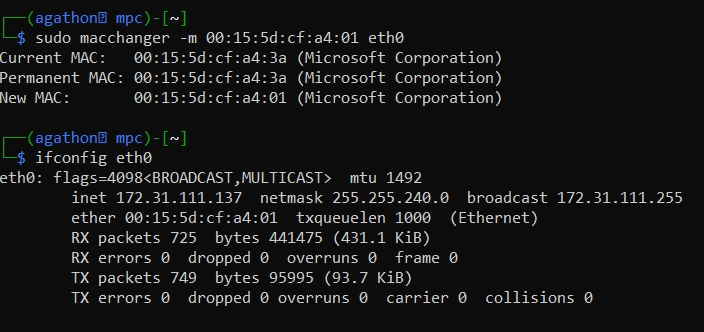
\includegraphics[width=0.75\textwidth]{images/10}
	\centering
	\caption{macspoofing: Änderung der MAC-Adresse von eth0}
\end{figure}

Bei erneuter Aufzeichnung des Netzwerk-Verkehrs zum Zielserver lässt sich nun die gerade geänderte 
MAC-Adresse (\texttt{00:15:5d:cf:a4:01}) in dem Ethernet-Header jedes Pakets wiederfinden.
(Siehe Abb. 11)

\begin{figure}[H]
	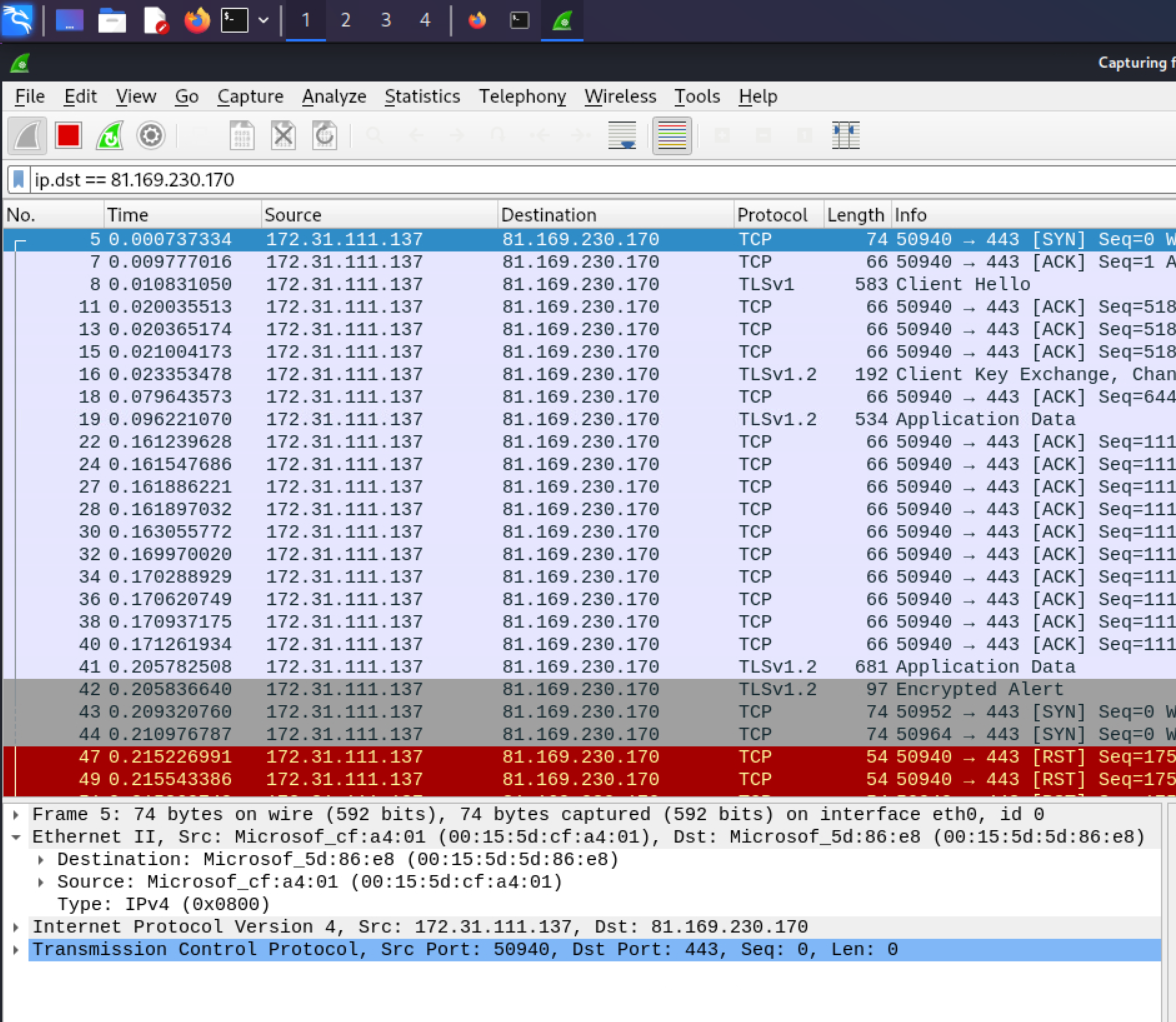
\includegraphics[width=0.75\textwidth]{images/11}
	\centering
	\caption{macspoofing: Veränderter Netzwerk-Verkehr}
\end{figure}

\newpage

\subsection{Schwachstellenscan II}

\subsubsection*{Aufgabenstellung}

Verwenden Sie das bei ParrotOS und Kali Linux vorinstallierte WPScan  (WordPress 
Vulnerability Scanner) und führen Sie einen Scan von https://nwsmooc.mooin.org durch. 
Erklären Sie die Ergebnisse.  

\begin{flushleft}
	Hinweise:	
\end{flushleft}


\begin{itemize}
	\item Es ist keine Registrierung beim Anbieter erforderlich. Durch eine Registierung würde man ein Token erhalten, um Schwachstellentests durchführen zu können. So ist die Aufgabe auf eine Informationssammlung beschränkt.
	\item Bei einem Test mit ParrotOS gab es zunächst eine Fehlermeldung, dass ein Update der Datenbank nicht möglich sei. Ein allgemeines Update
		(\texttt{sudo apt-get update \&\& apt-get upgrade}) konnte dieses Problem beseitigen.
\end{itemize}

Sollten Sie Mac oder Linux verwenden, dann installieren Sie WPScan direkt von Github. 
Sollten Sie keine Möglichkeit zur Durchführung dieses Aufgabenteils finden, sprechen 
Sie die Betreuenden auf eine Ersatzaufgabe an.

\subsubsection*{Antwort}

\texttt{wpscan} ist ein Open-Source-Tool, das für die Sicherheitsüberprüfung von 
WordPress-Websites entwickelt wurde, um potenzielle Schwachstellen und Sicherheitsprobleme in 
diesen zu erkennen. Es ermöglicht die Analyse von WordPress Webseiten nach eigenen Angaben 
seit über 10 Jahren und hat in dieser Zeit einen Katalog von mehr als 43000 Core, Plugin oder 
Theme Schwachstellen aufgebaut (Quelle \url{https://wpscan.com}). Ein Scan einer Webseite ist 
direkt von der \url{wpscan.com} Webseite möglich, oder vom eigenen Client aus mit dem CLI 
Programm \texttt{wpscan}.

Man bietet neben der kostenfreien Version für ``Researcher'' mit maximalen 25 API Calls pro 
Tag, auch eine nicht kostenlose Enterprise Version an.

Die Nutzung ist dabei gänzlich einfach. Der einfache Quick Scan wird durch den Aufruf 
\texttt{wpscan –url <webseite>} aufgerufen. Dabei erhielten wir jedoch statt eines 
Ergebnisses eine Fehler-Meldung über einen 403-Status-Code. (Siehe Abb. 12)

\begin{figure}[H]
	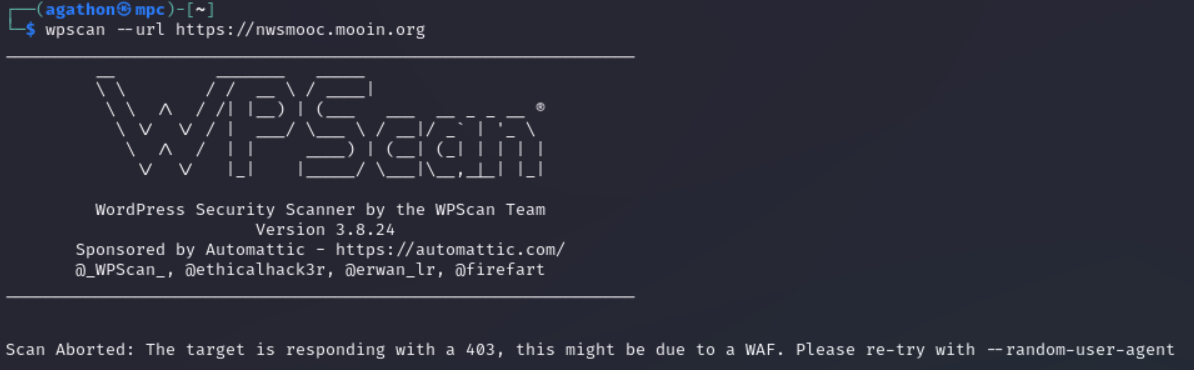
\includegraphics[width=0.75\textwidth]{images/12}
	\centering
	\caption{wpscan: Fehler}
\end{figure}

Der hier referenzierte HTTP-Statuscode bedeutet, dass der Server den Zugriff auf die 
angefragte Seite verweigert. Dies kann auf fehlende Zugriffsberechtigungen oder eine Web 
Application Firewalls (WAF) hinweisen. Eine WAF soll Websites und Webanwendungen vor 
böswilligen Anfragen und Zugriffen schützen, indem sie den Datenverkehr zwischen dem Client 
und dem Webserver analysiert, um Angriffe wie SQL-Injection, Cross-Site Scripting (XSS) und 
Distributed Denial of Service (DDoS) zu erkennen und zu blockieren. Sie verwendet dazu Regeln 
und Signaturen und ist ein wichtiger Bestandteil um die Sicherheit einer Webseite zu 
gewährleisten und Angriffe auf Anwendungsebene abzuwehren.

Der Parameter \texttt{--random-user-agent} aus dem gegebenen Hinweis versucht diesen 
Sicherheitsmechanismus zu umgehen, indem automatisch zufällige Benutzer-Agenten für jede 
HTTP-Anfrage, die es während des Scans an die WordPress-Website sendet, generiert um diese 
Anfragen weniger auffällig und weniger vorhersehbar zu gestalten um nicht automatisiert zu 
wirken. Da wir kein Bot-Netz oder ähnliches verwenden, ist die IP-Adresse der Anfragen jedoch 
die gleiche. Dies schien jedoch nicht von der Firewall verhindert zu werden, denn mit jenem 
Parameter lässt sich ein Scan durchführen. (Siehe Abb. 13)

\begin{figure}[H]
	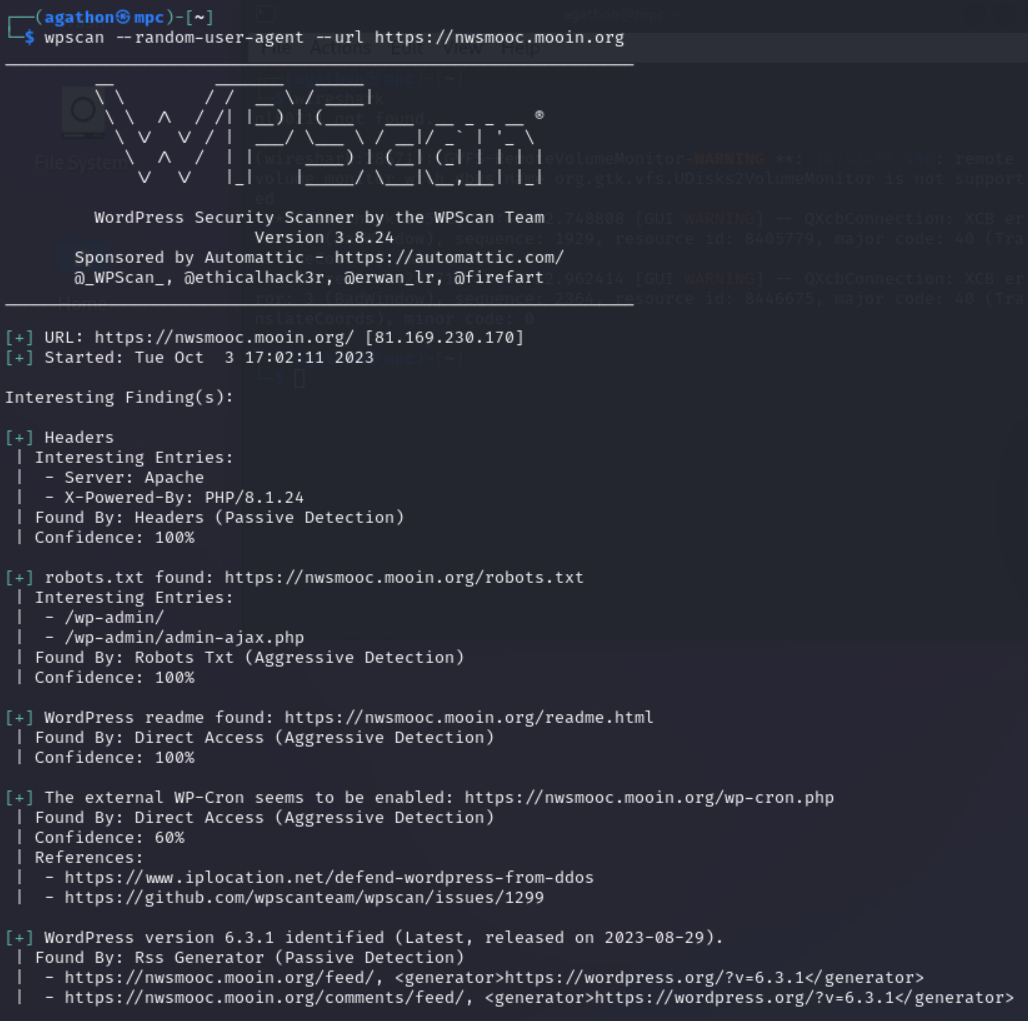
\includegraphics[width=0.75\textwidth]{images/13}
	\centering
	\caption{wpscan: Ergebnis 1/2}
\end{figure}

In einer detaillierten Ansicht erhalten wir Informationen ausgegeben, die durch den Scan 
gewonnen wurden konnte. (Siehe Abb. 14)

\begin{itemize}
	\item Ein Apache Webserver mit der PHP Version 8.1.24 liefert die Webseite aus (diese ist aktuell – Release Datum 28.09.2023)
	\item WordPress ist installiert in der Version 6.3.1 (ebenfalls zum Zeitpunkt des Scans 
		aktuell mit Release Datum 29.08.2023). Ein RSS Feed ist vorhanden unter angegebener 
		URL.
	\item \texttt{robots.txt} (Anweisungen/Berechtigungen für Web-Crawler von Suchmaschinen) 
		und Wordpress-Readme sind vorhanden – Ausgabe mit Pfad
	\item WP-Cron ist aktiviert – dies lässt eine automatisierte Aktualisierung der Software-Komponenten der Wordpress-Installation annehmen
	\item twentysixteen ist das installierte Wordpress-Theme (ebenfalls zum Zeitpunkt des Scanns aktuell mit Release Datum 29.03.2023). Eine eigene Readme ist unter der angegebenen URL zu erreichen. Eine kurze Description und eine Style URI sind auslesbar.
	\item Ein Plugin-Scan mit passiver Scan-Methode findet keine installierten Plugins.
	\item Es werden keine scanbaren Config-Backups gefunden
\end{itemize}

\begin{figure}[H]
	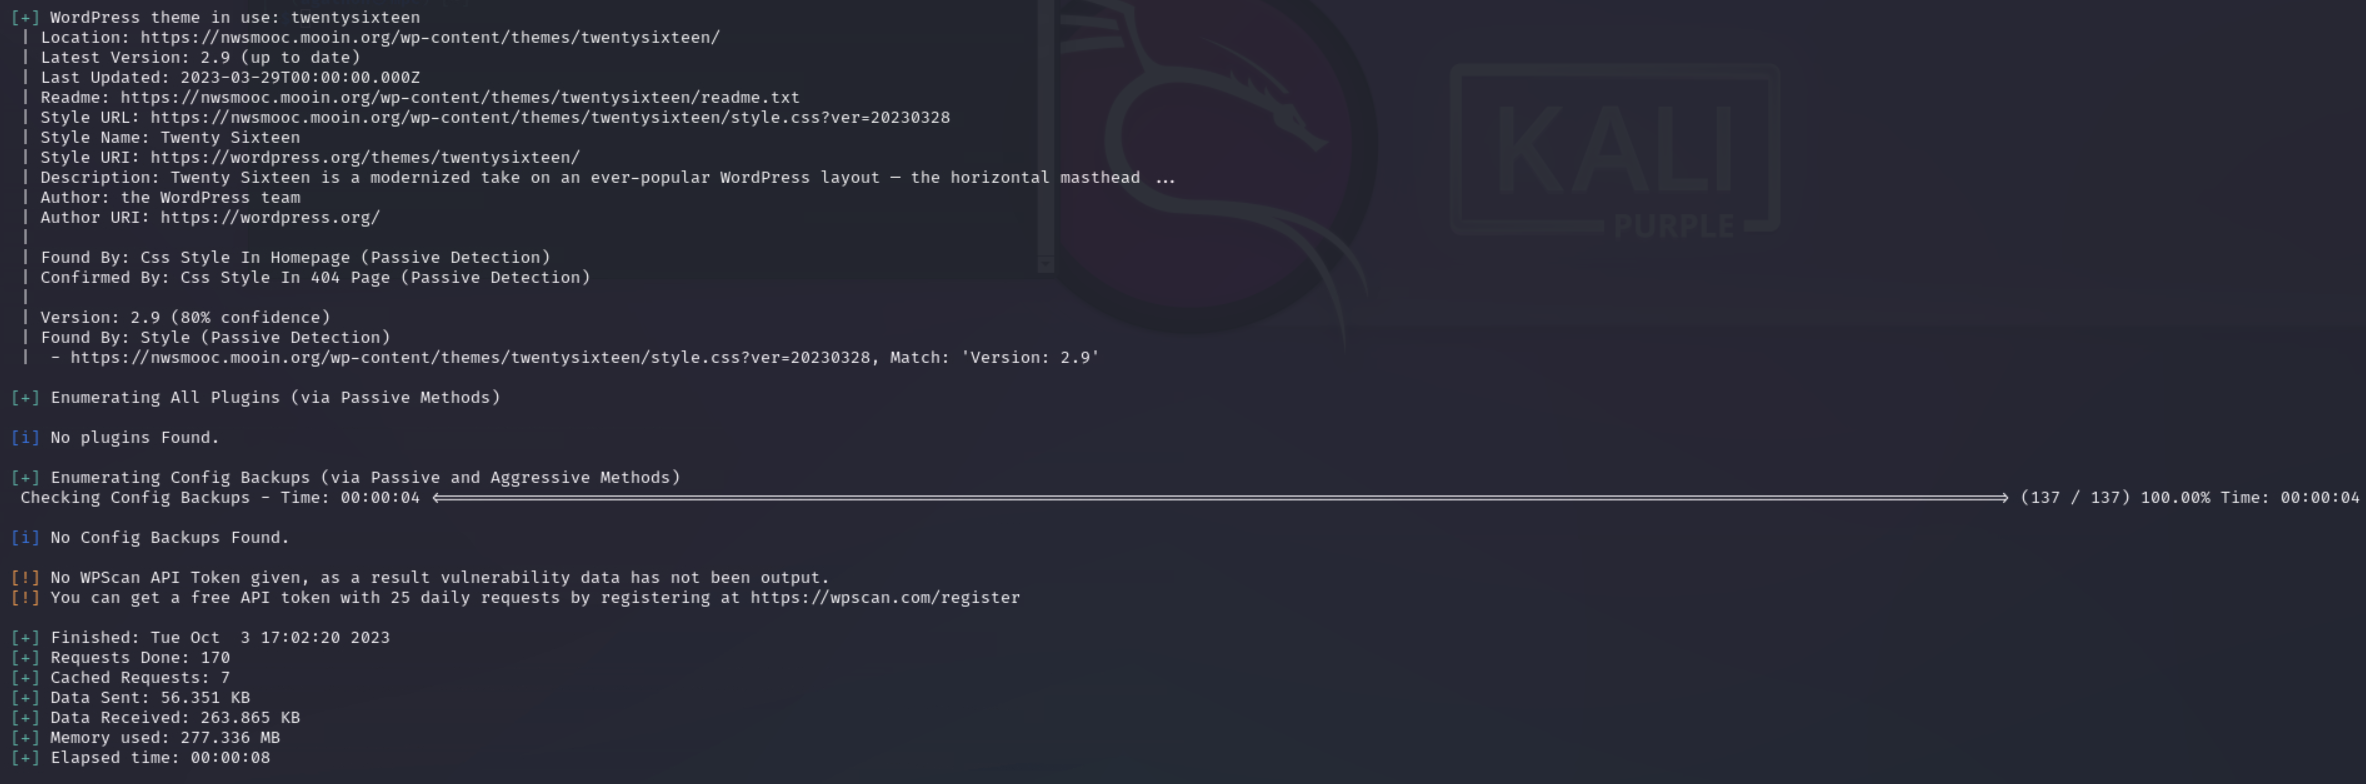
\includegraphics[width=0.75\textwidth]{images/14}
	\centering
	\caption{wpscan: Ergebnis 2/2}
\end{figure}

Da wir, wie in der Aufgabenstellung beschrieben, keine Registrierung beim \texttt{wpscan}
Anbieter durchführen und daher keinen API-Key besitzen, endet unser Scan an dieser Stelle.

\newpage

\subsection{Google-Hacking}

\subsubsection*{Aufgabenstellung}

Mit "Google Hacking" ist gemeint, dass man die Google Suche zum Auffinden von
Softwareinstallationen mit Schwachstellen nutzen kann. Eine Sammlung von Beispielen ist 
bei \url{https://www.exploit-db.com/google-hacking-database/} zu finden. Erklären Sie 
anhand von drei selbstgewählten Beispielen, was man damit herausfinden kann.
Achtung: Firefox und Google Chrome warnten teilweise beim Aufruf der Seite und bezeichneten diese als riskant. Man kann die Seite aber aus einem Browser innerhalb von Kali Linux oder ParrotOS aufrufen, dann kommt keine Warnung.

\subsubsection*{Antwort}

Innerhalb der Exploit-Datenbank haben wir uns drei, unserer Meinung nach, besonders 
interessante Beispiele ausgesucht.

Das erste unserer Beispiele beruht auf dem Prinzip Google-Filter zu verwenden um von 
Google indexierte Dateien mit bestimmten Namen oder Dateiendungen zu finden. So können zum 
Beispiel falsch konfigurierte Web-Server aus Versehen vertrauliche Daten öffentlich 
zugänglich machen. Ein interessantes Beispiel ist hierbei nach rohen SQL-Backups zu 
suchen. Diese könnten, bei schlechten Sicherheitsmaßnahmen des Servers, rohe Nutzerdaten 
enthalten und somit entweder einen Angriff auf die betroffenen Accounts ermöglichen oder 
weiter verwendet werden um Zugriff auf andere, möglicherweise interessantere, Systeme zu 
erlangen. (Siehe Abb. 15)

\begin{figure}[H]
	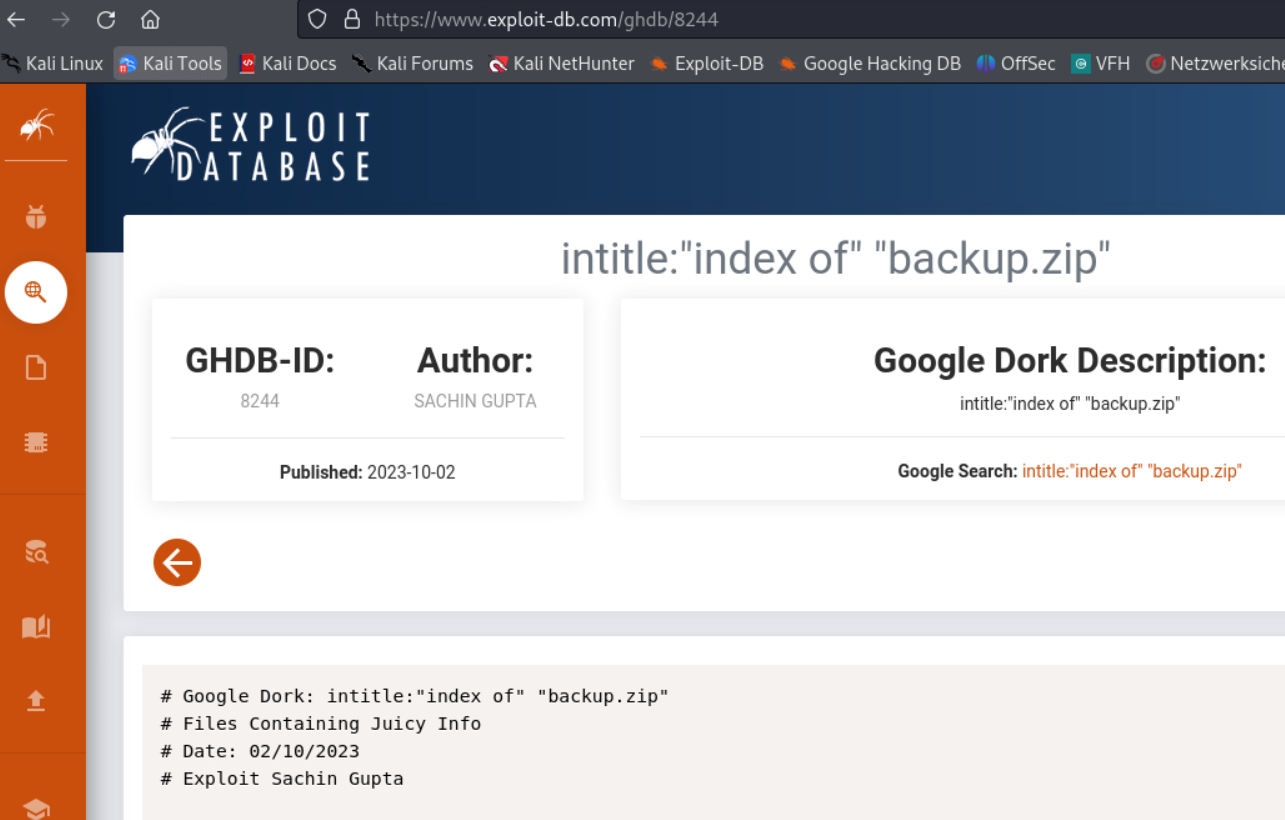
\includegraphics[width=0.75\textwidth]{images/15}
	\centering
	\caption{Google Hacking: Backup: Schwachstelle}
\end{figure}

Bei einer Google-Suche nach Dateiverzeichnissen, die eine Datei namens backup.zip enthalten
sind wir sofort auf einen Web-Server gestoßen, bei dem sowohl eine backup.zip und eine backup.sql
Datei versehentlich veröffentlicht wurden. (Siehe Abb. 16 \& 17)

\begin{figure}[H]
	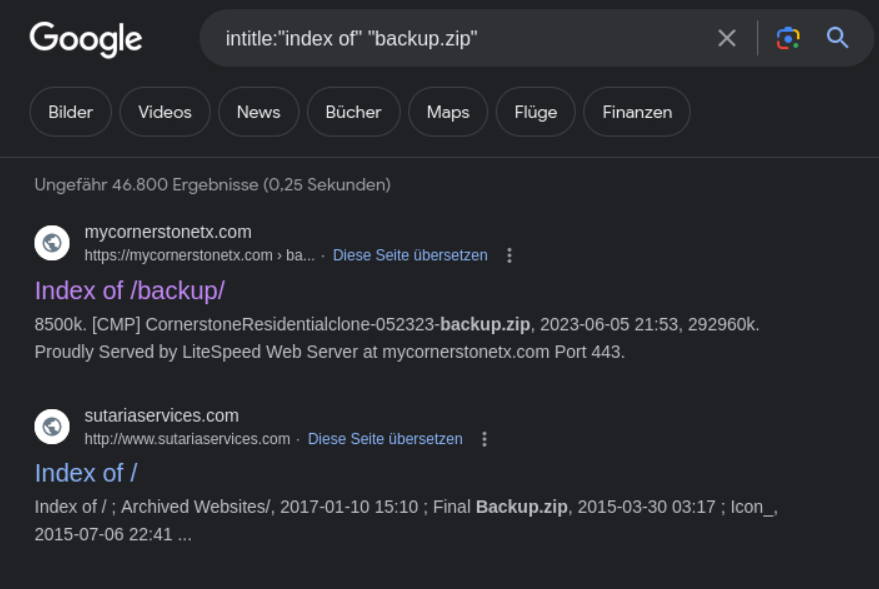
\includegraphics[width=0.75\textwidth]{images/16}
	\centering
	\caption{Google Hacking: Backup: Google Suche}
\end{figure}

\begin{figure}[H]
	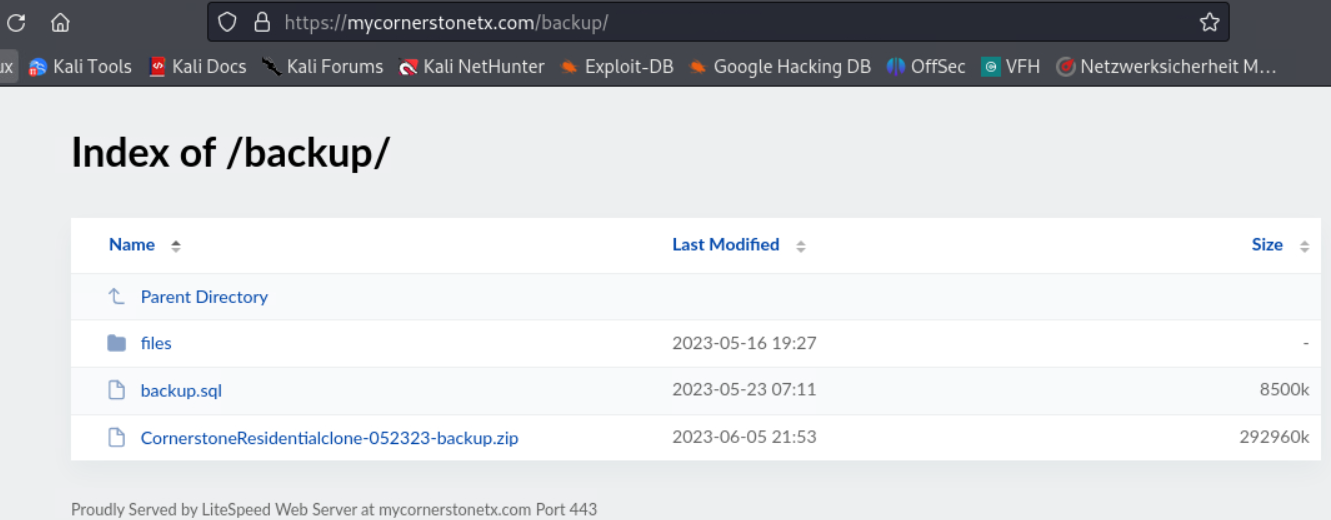
\includegraphics[width=0.75\textwidth]{images/17}
	\centering
	\caption{Google Hacking: Backup: Ergebnis}
\end{figure}

---

Das zweite unserer Beispiele ist die Suche nach Webseiten die Tokens oder ähnlich vertrauliche 
Informationen im Klartext enthalten. Dies ist ein besonders hohes Risiko bei Seiten, die 
Quellcode enthalten (Wie z.B. Pastebin oder GitHub). Das Beispiel in unserer Abbildung 
sucht nach Tokens auf öffentlich-zugänglichen Pastebin-Seiten.

Bei einer Suche nach pastebin.com Seiten, die entweder einen Benutzernamen, ein Passwort oder
einen Schlüssel enthalten haben wir ebenfalls sofort Ergebnisse erzielen können.
(Siehe Abb. 18 \& 19)

\begin{figure}[H]
	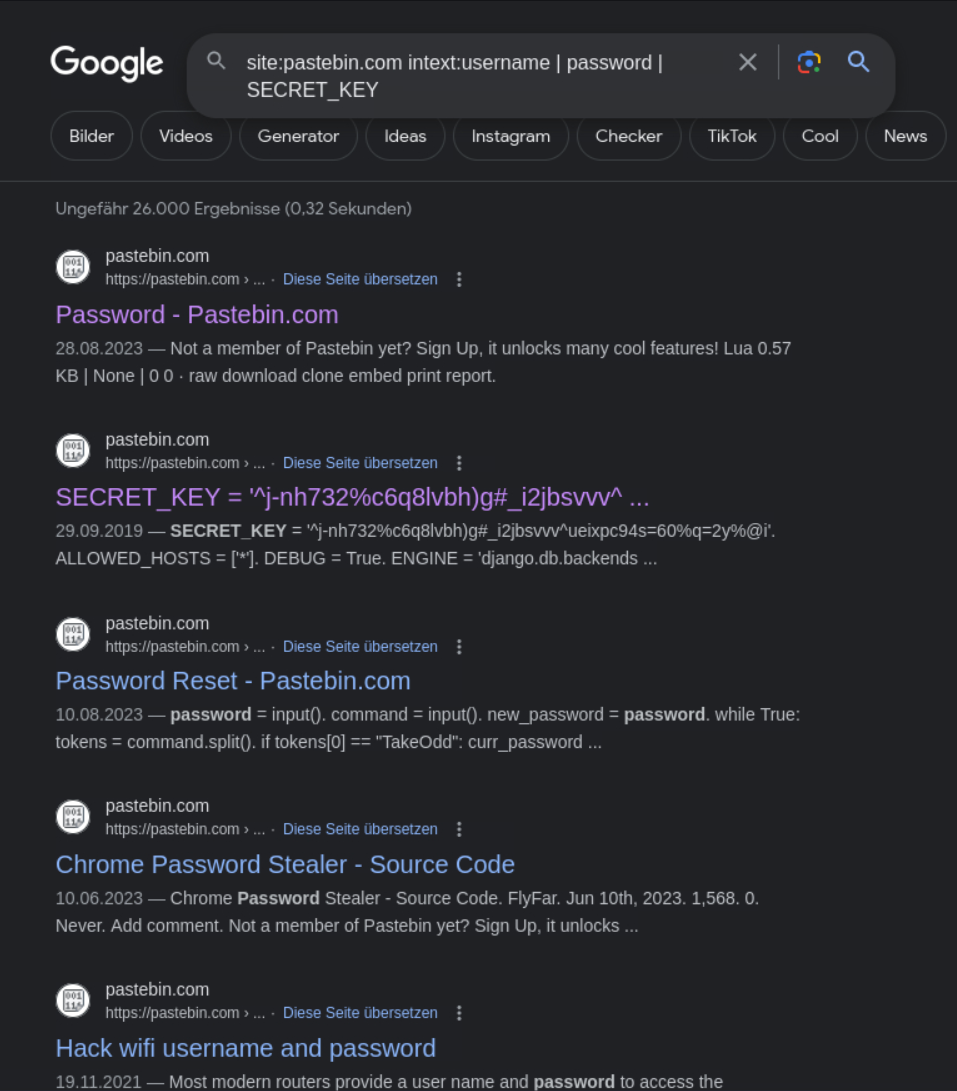
\includegraphics[width=0.75\textwidth]{images/18}
	\centering
	\caption{Google Hacking: Tokens: Suche}
\end{figure}


\begin{figure}[H]
	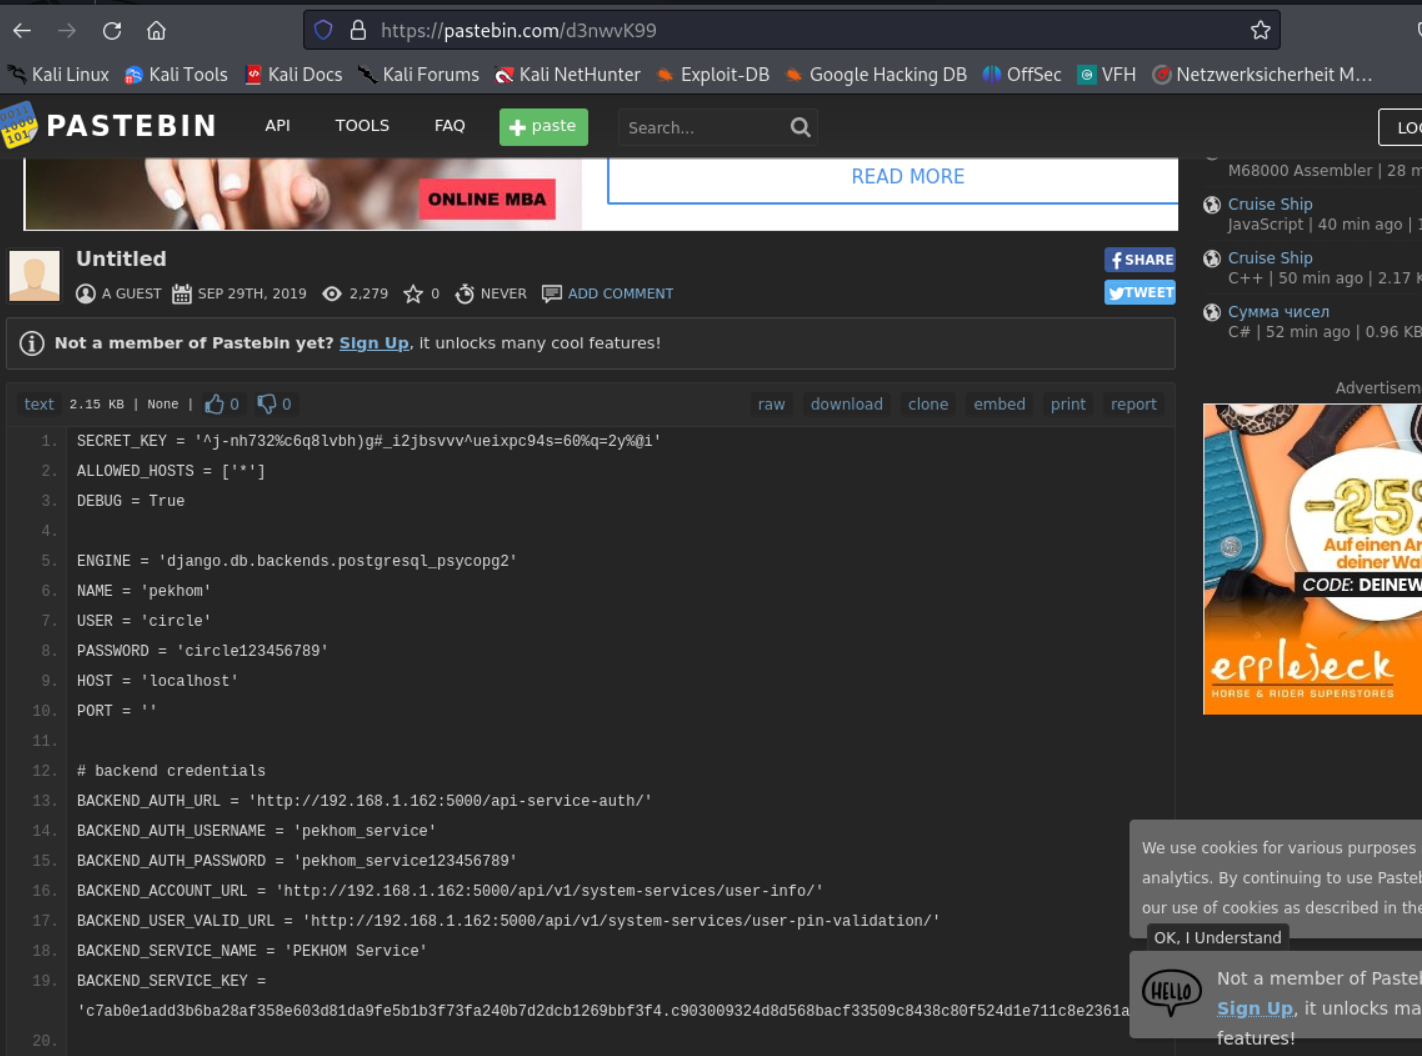
\includegraphics[width=0.75\textwidth]{images/19}
	\centering
	\caption{Google Hacking: Tokens: Ergebnis}
\end{figure}

---

Die letzte, und wohl kritischte Schwachstelle, die wir im Rahmen dieser Aufgabe gefunden 
haben, ist eine SQL-Injektion durch einen falsch programmierten PHP-Web-Server. Die Exploit-Datenbank
listet hierzu drei typische Suchbefehle, wobei wir uns für den ersten entschieden haben, da er
die größte Erfolgswahrscheinlichkeit hatte. (Siehe Abb. 20 \& 21)


\begin{figure}[H]
	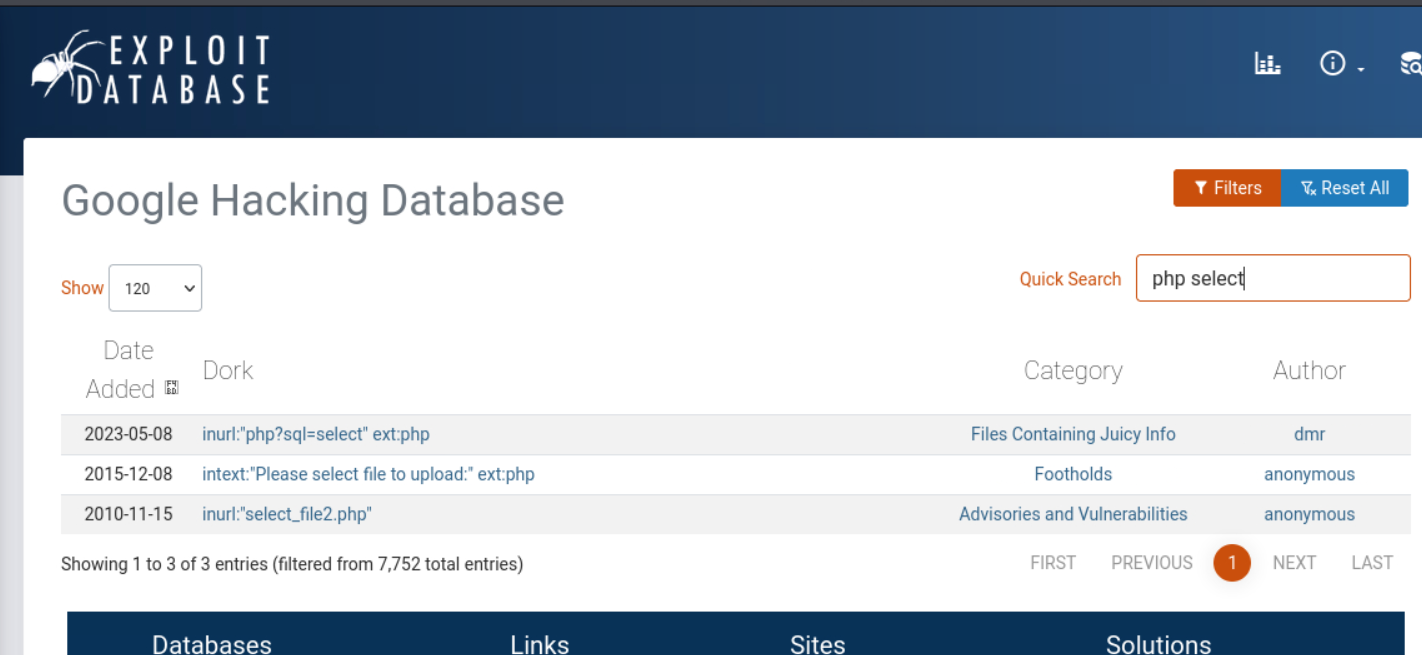
\includegraphics[width=0.75\textwidth]{images/20}
	\centering
	\caption{Google Hacking: SQL Injektion: Schwachstelle}
\end{figure}

\begin{figure}[H]
	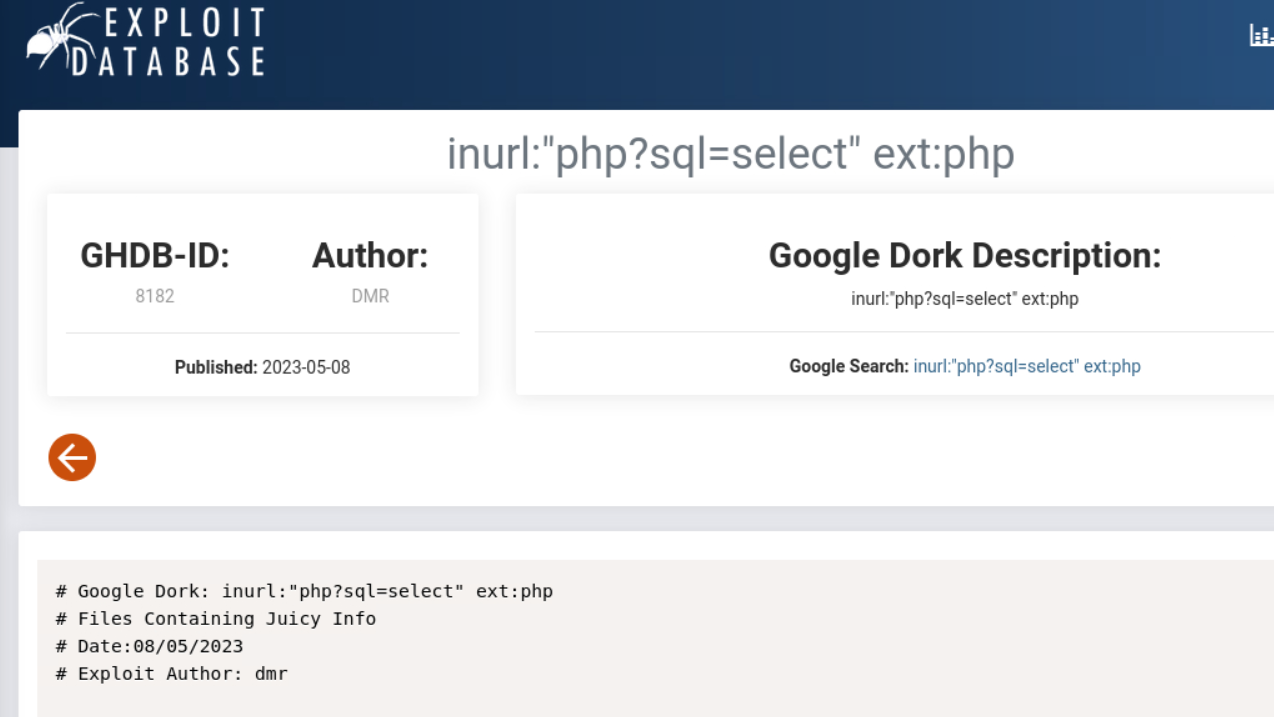
\includegraphics[width=0.75\textwidth]{images/21}
	\centering
	\caption{Google Hacking: SQL Injektion: Schwachstelle}
\end{figure}

Bei einer Google-Suche, kam neben einem PHP-Tutorial, sofort eine öffentliche PHP-Datei,
die rohe SQL-Befehle als Query-Parameter annimmt. (Siehe Abb. 22)

\begin{figure}[H]
	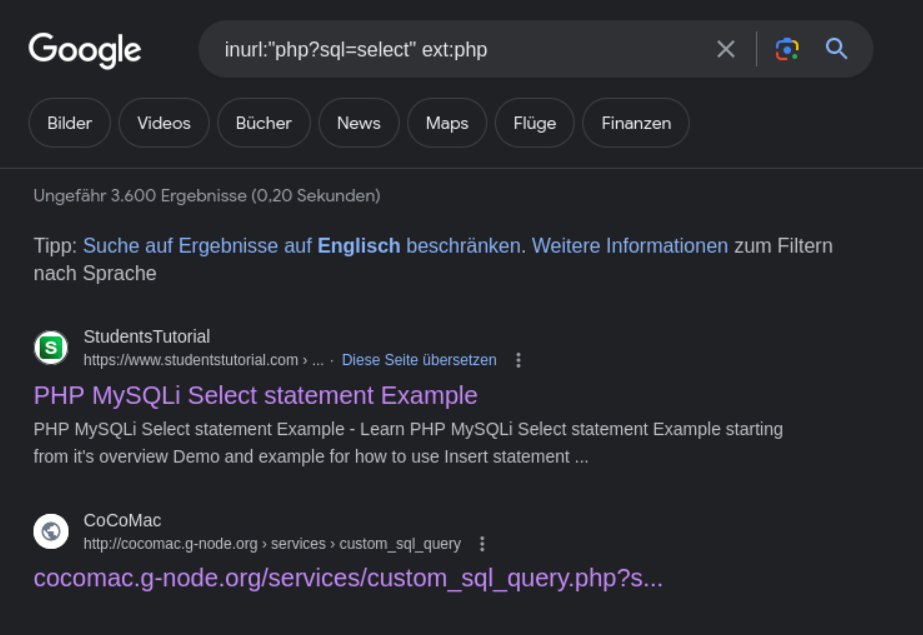
\includegraphics[width=0.75\textwidth]{images/22}
	\centering
	\caption{Google Hacking: SQL Injektion: Suche}
\end{figure}

Beim Aufruf dieser Seite wurden ursprünglich lediglich nicht vertrauliche Datensätze geladen,
allerdings konnten wir zeigen, dass das SQL-Statement austauschbar ist, in dem wir (wie in Abb. 23 gezeigt)
einen \texttt{show tables;} Befehl ausgeführt haben um die verschiedenen Tabellen in der angebundenen Datenbank
aufzulisten.

\begin{figure}[H]
	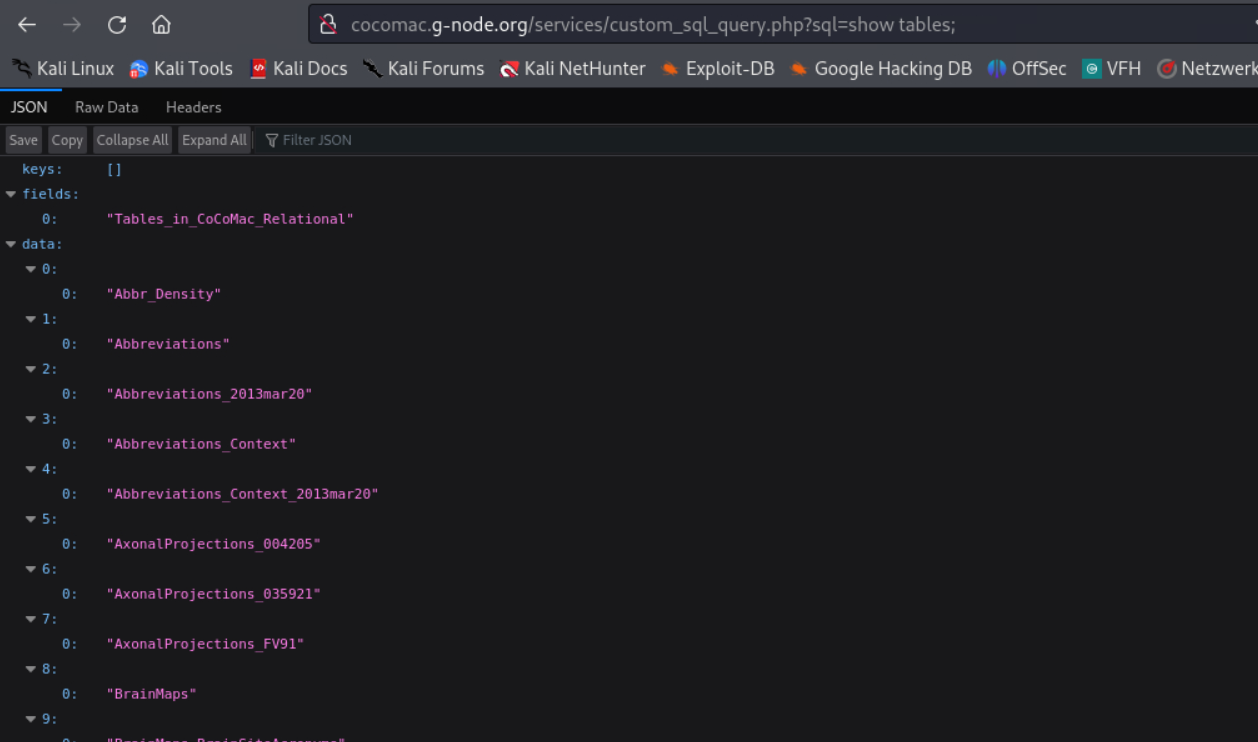
\includegraphics[width=0.75\textwidth]{images/23}
	\centering
	\caption{Google Hacking: SQL Injektion: Ergebnis}
\end{figure}

Diese Schwachstelle könnte nun genutzt werden, um Beispielsweise neue Admin-Nutzer anzulegen,
bestehende zu löschen, die Daten innerhalb der Datenbank zu manipulieren oder abzufragen etc.
Über die Abfrage nach weiteren Tabellen hinaus, haben wir keine Befehle ausgeführt um strafrechtliche
Probleme zu vermeiden.

\end{document}
